%\documentclass{article}
\documentclass[]{article}
\usepackage{bm}
\usepackage{amsmath}
\usepackage{amsfonts}
\usepackage{natbib}
\usepackage{graphicx}
\usepackage{placeins}
\usepackage{caption}
\usepackage{subcaption}
\bibliographystyle{unsrtnat}


\begin{document}
	
\section{Update - February 24th 2021}	
\FloatBarrier
\subsection{Multipliers}

\begin{figure}
	\centering
	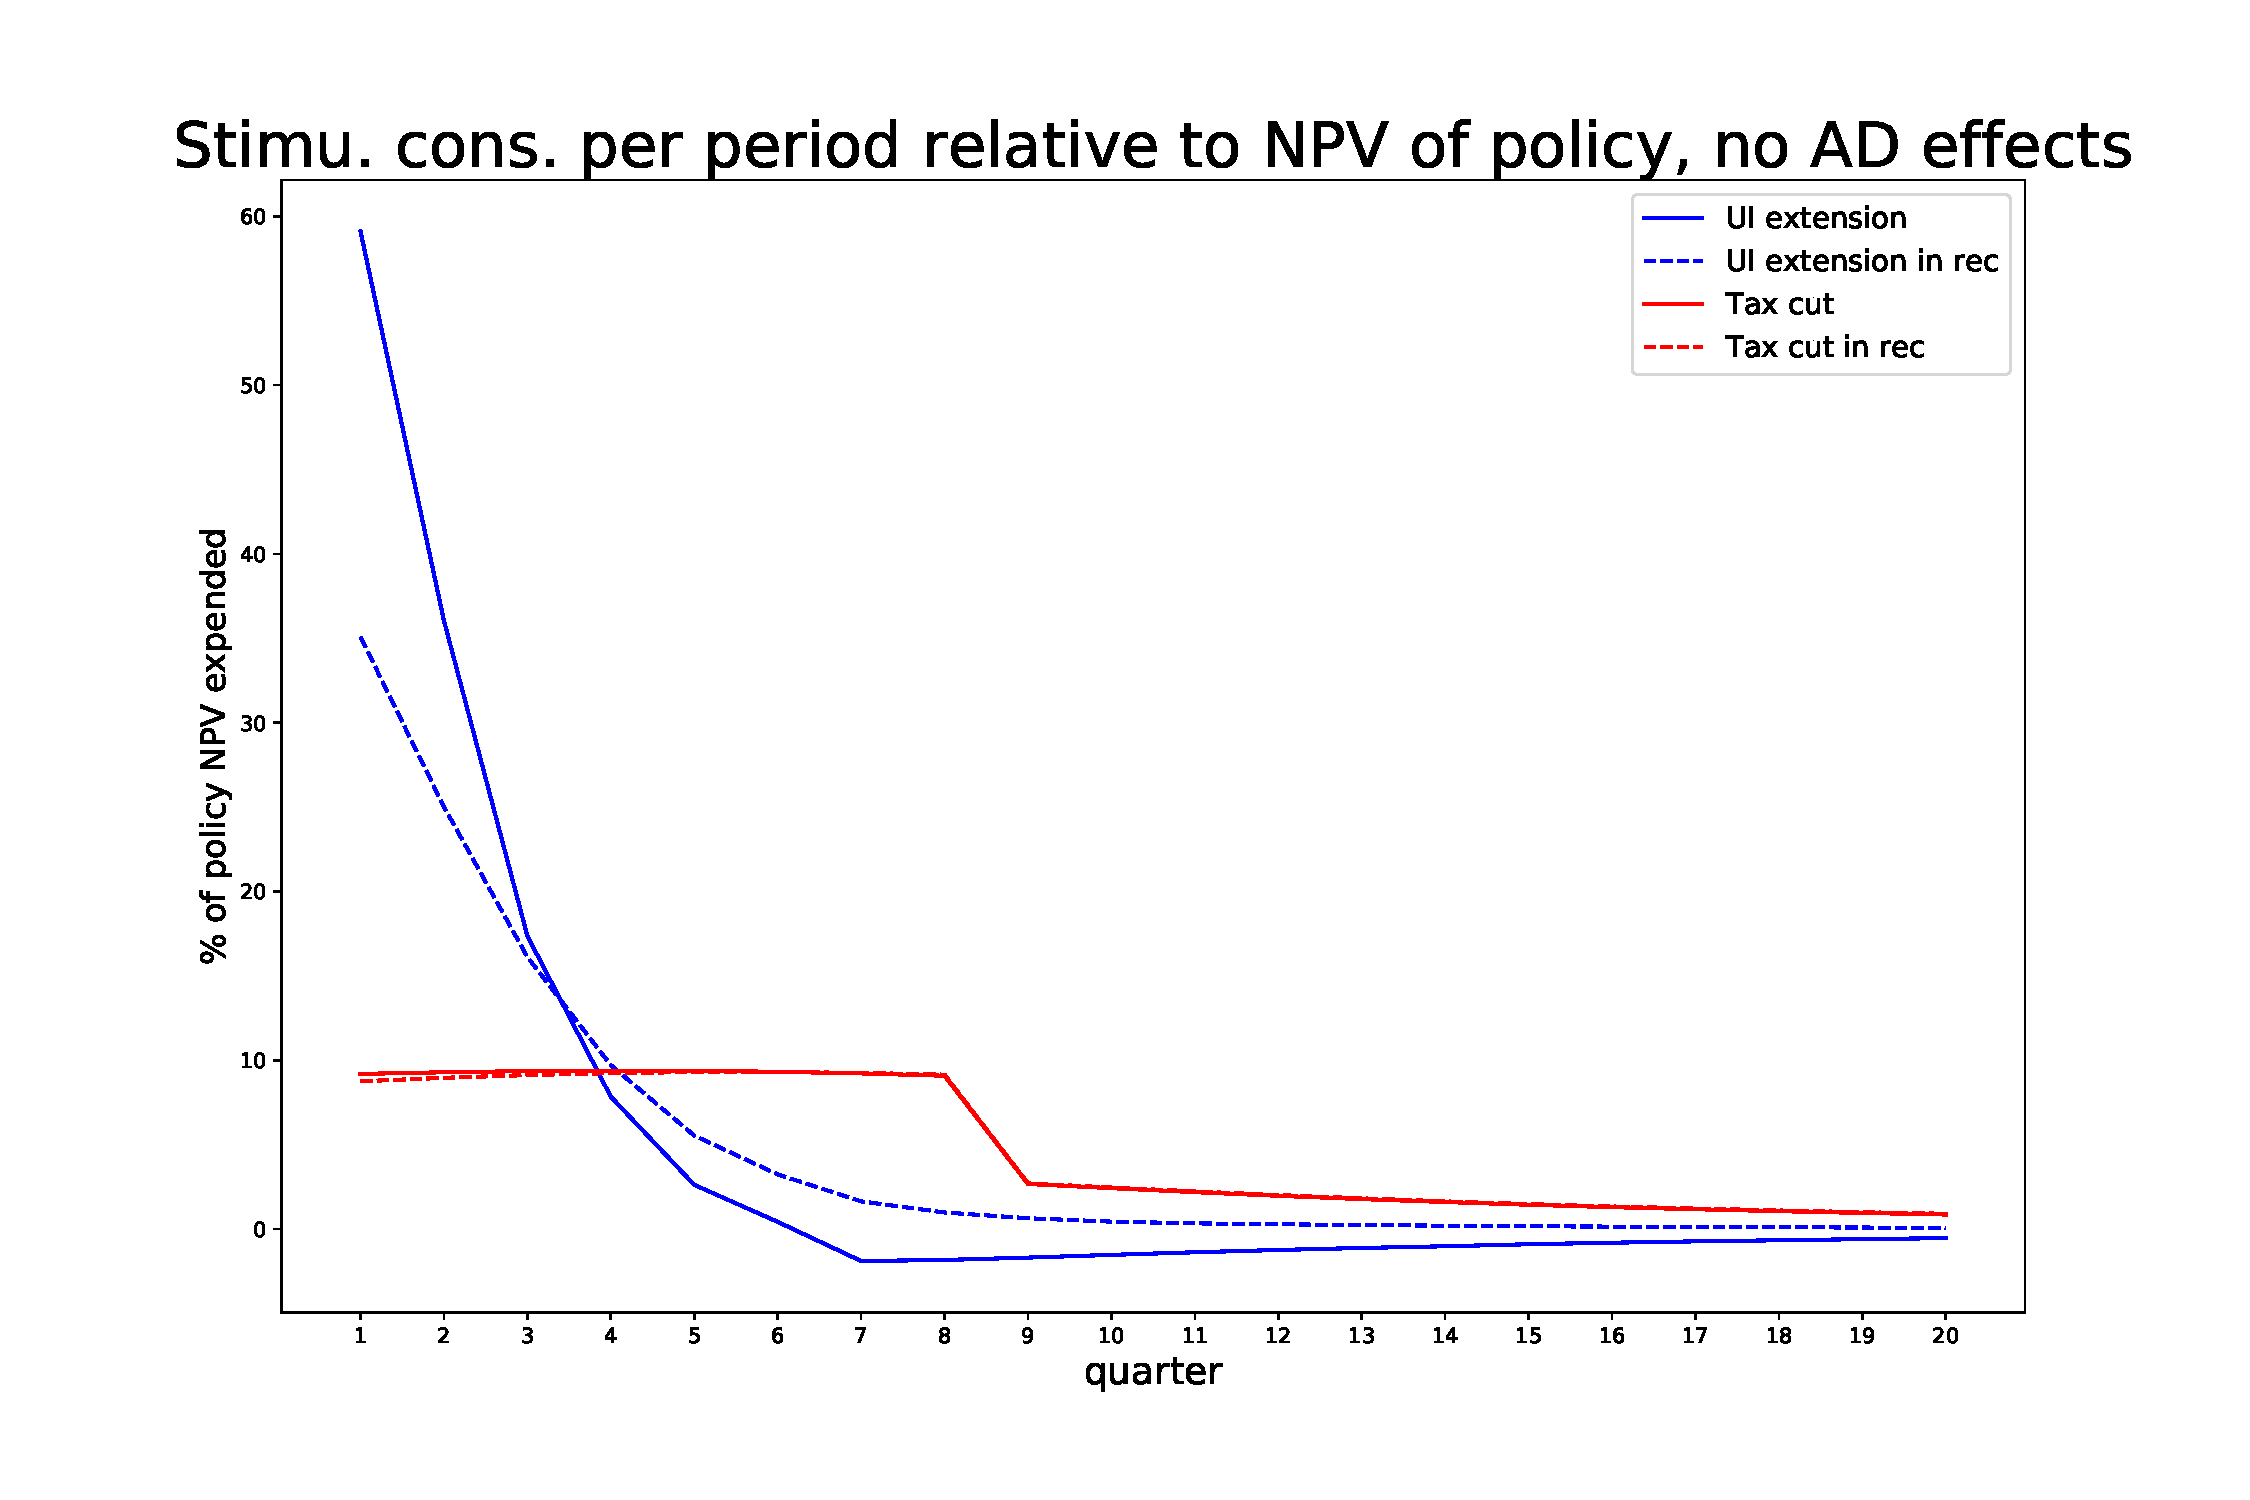
\includegraphics[width=\linewidth]{../Full_Run_with_UI_Ext/NPV_Multiplier_no_AD}
	\caption{}
	\label{fig:npvmultipliernoad}
\end{figure}


\begin{figure}
	\centering
	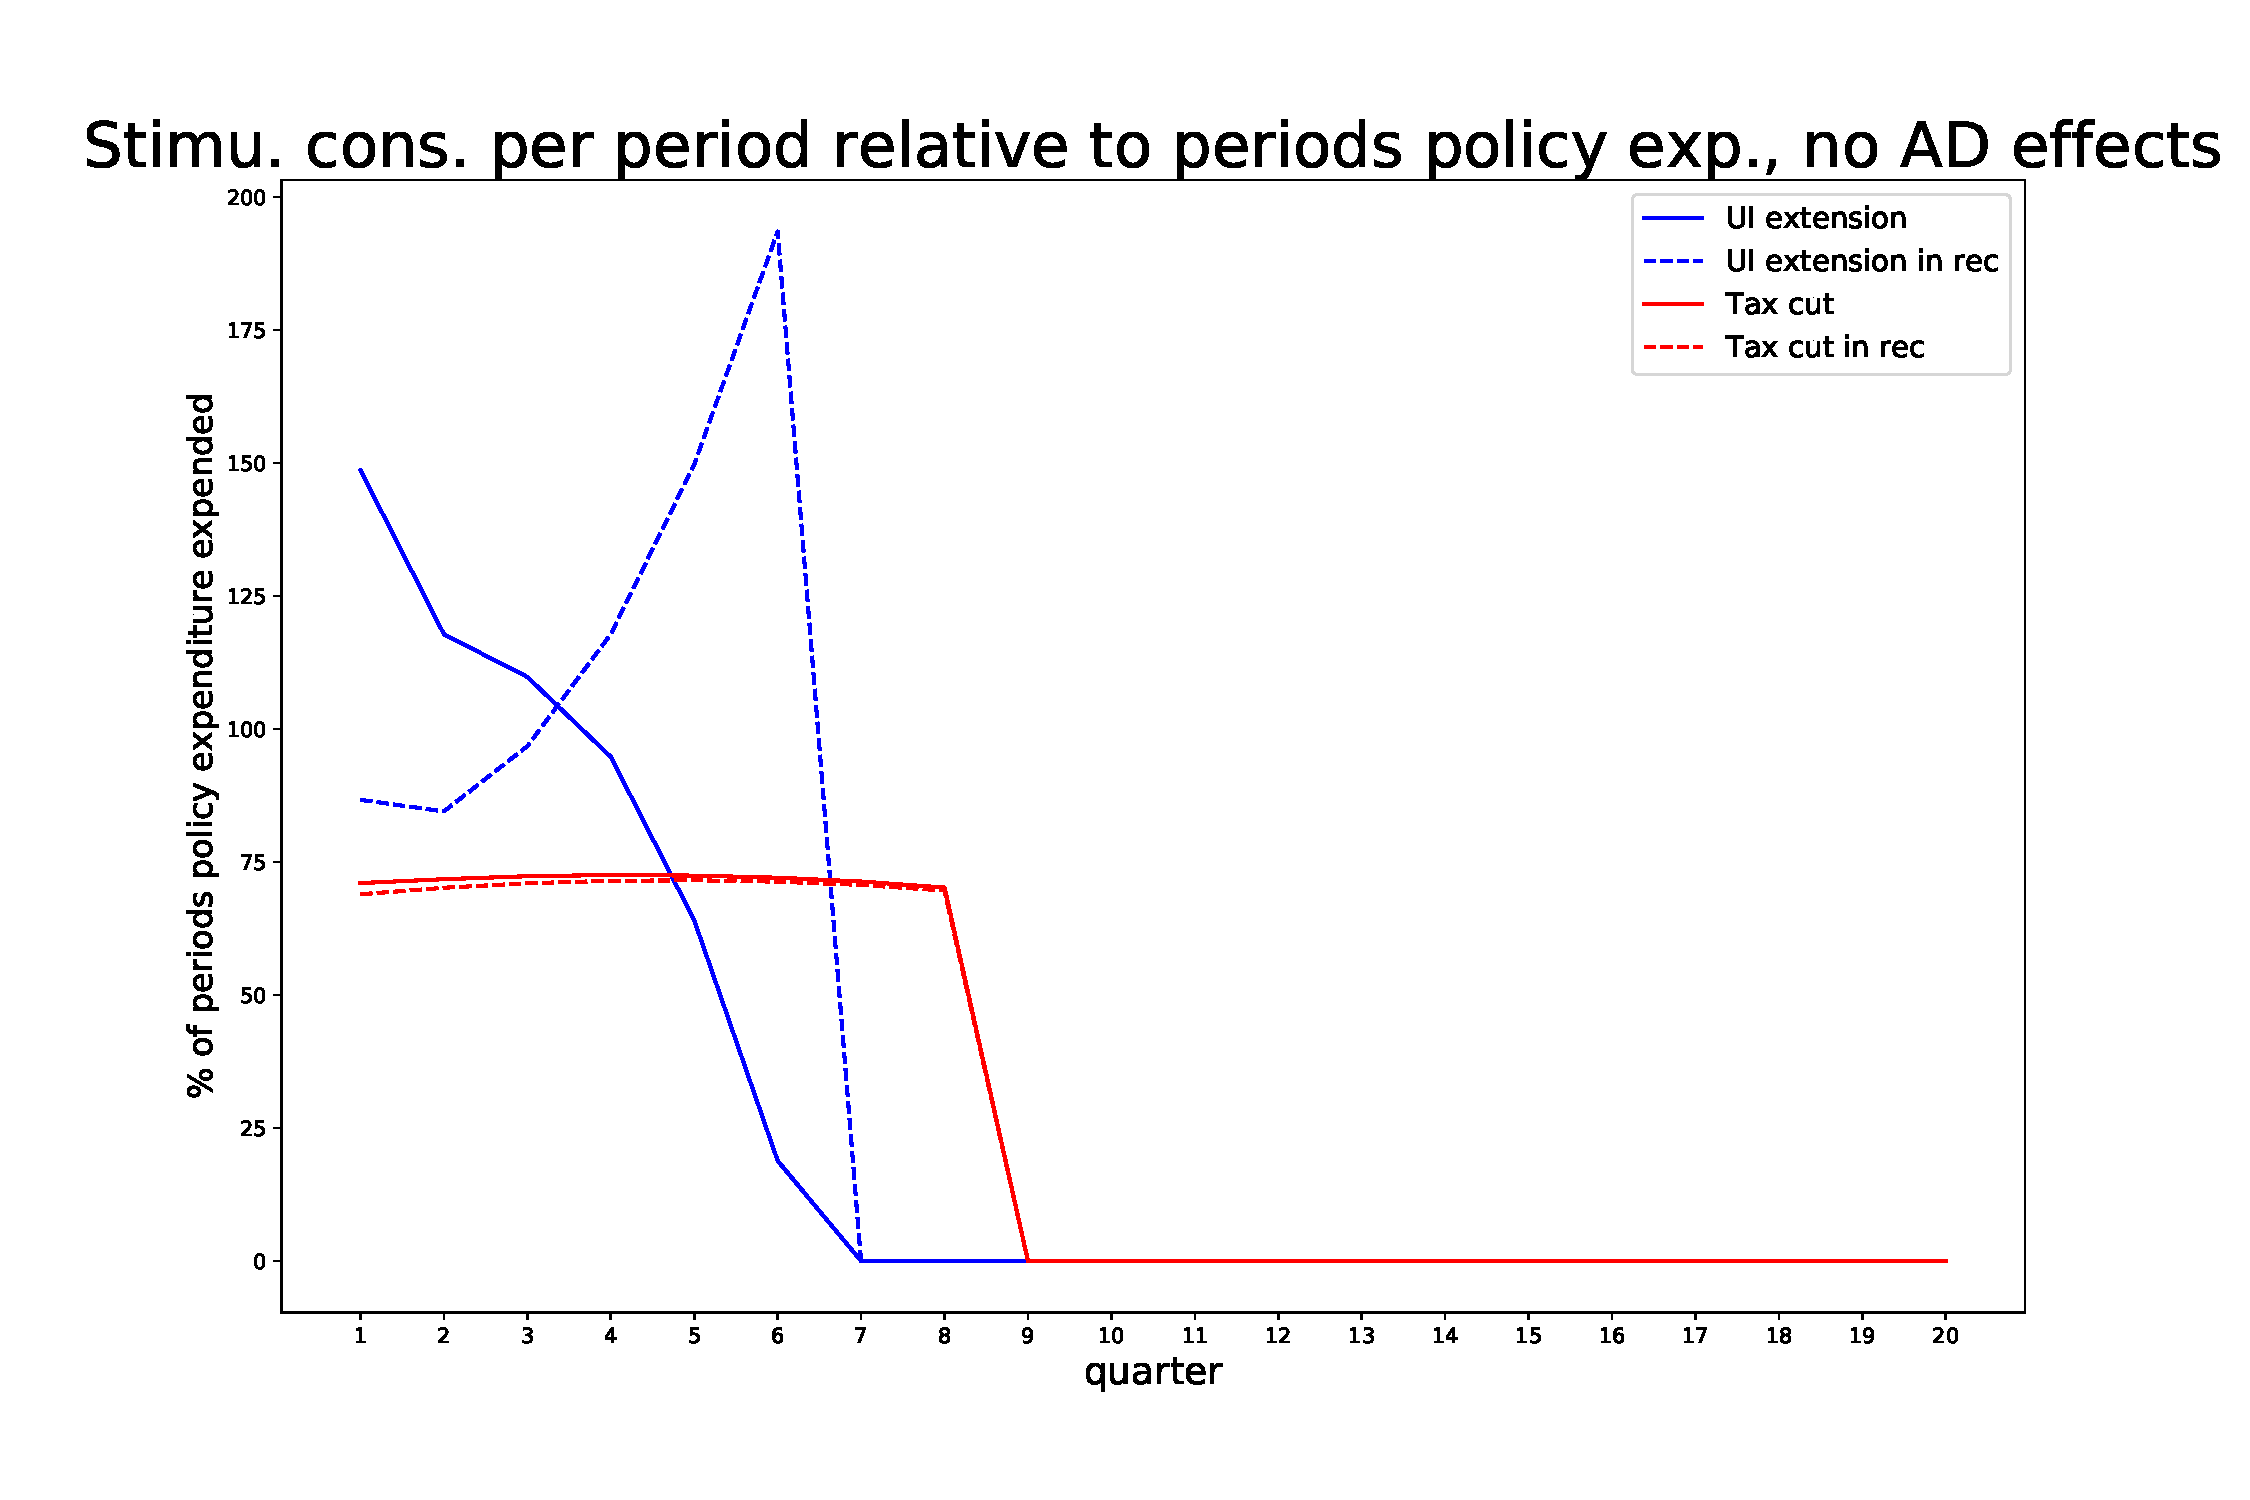
\includegraphics[width=\linewidth]{../Full_Run_with_UI_Ext/Period_Multiplier_no_AD}
	\caption{}
	\label{fig:periodmultipliernoad}
\end{figure}


\FloatBarrier
\subsection{Continuation probability linked to business cycle state}
\begin{itemize}
	\item Figure \ref{fig:taxcutrecessionnoadeffects}: No AD effects
	\item Consider either 8q or 16 tax cut (black lines)
	\item Simulations: Conditional on recesssion lasting at least 9q (otherwise: probability of continuation only when recession in q8 is meaningless.)
	\item Consumption in the case of tax cut only occuring 8q long
	\subitem - Blue:  Zero probability of continuation of tax cut after 8q
	\subitem - Green: 50\% probability of continuation of tax cut after 8q (independent of business cycle)
	\subitem - Red:   50\% probability of continuation of tax cut after 8q only when recession in q8: This curve is upward sloping as with the recession staying on it becomes more and more likely that tax cut will be extended
	\item Consumption in the case of tax cut being continued after q8
	\subitem - Green:  50\% probability of continuation of tax cut after 8q (independent of business cycle)
	\subitem - Red:    50\% probability of continuation of tax cut after 8q only when recession in q8
	\subitem - Orange: 100\% probability of continuation of tax cut after 8q only when recession in q8
	\item Conclusion: Continuing the payroll tax cut even when recession ends does not boost consumption by much (except during first quarters) (see diff red green line). More stimulating is a guarantee to extend the tax cut in case of an ongoing recession.
	\item Figure \ref{fig:taxcutrecessionadeffects}: same but with AD effects
\end{itemize}
	
\begin{figure}
	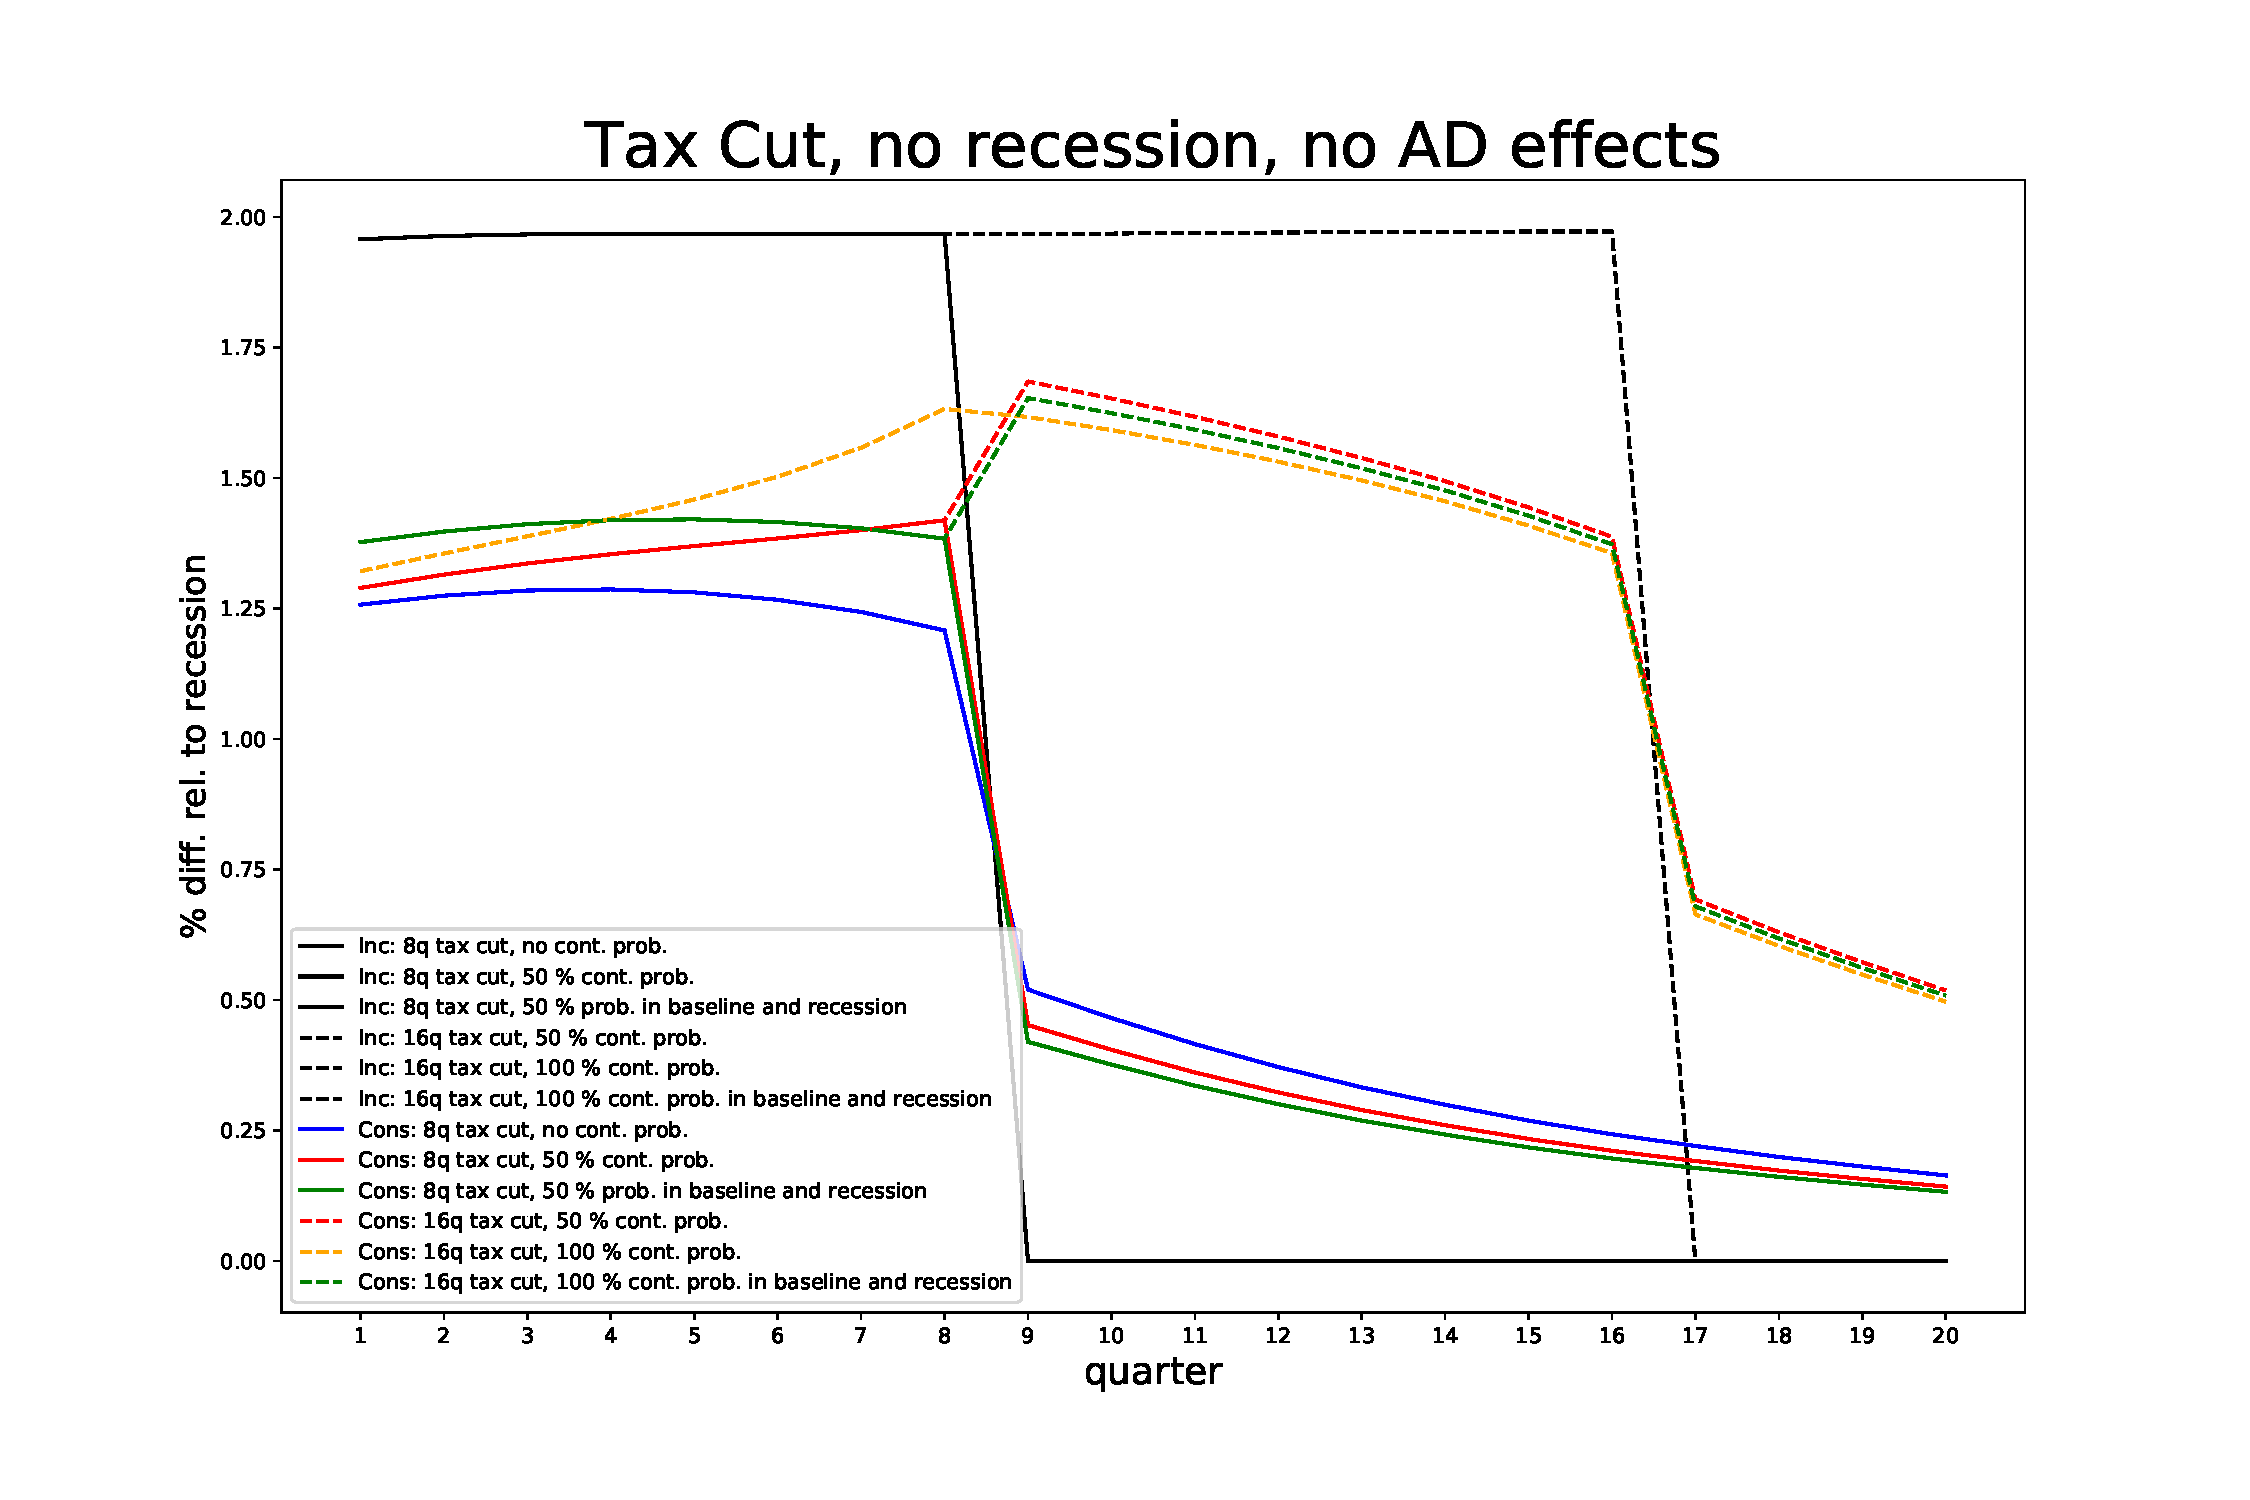
\includegraphics[width=1\linewidth]{../Continuation_Prob_Experiments/tax_cut_recession_no_AD_effects}
	\caption{}
	\label{fig:taxcutrecessionnoadeffects}
\end{figure}
	
\begin{figure}
	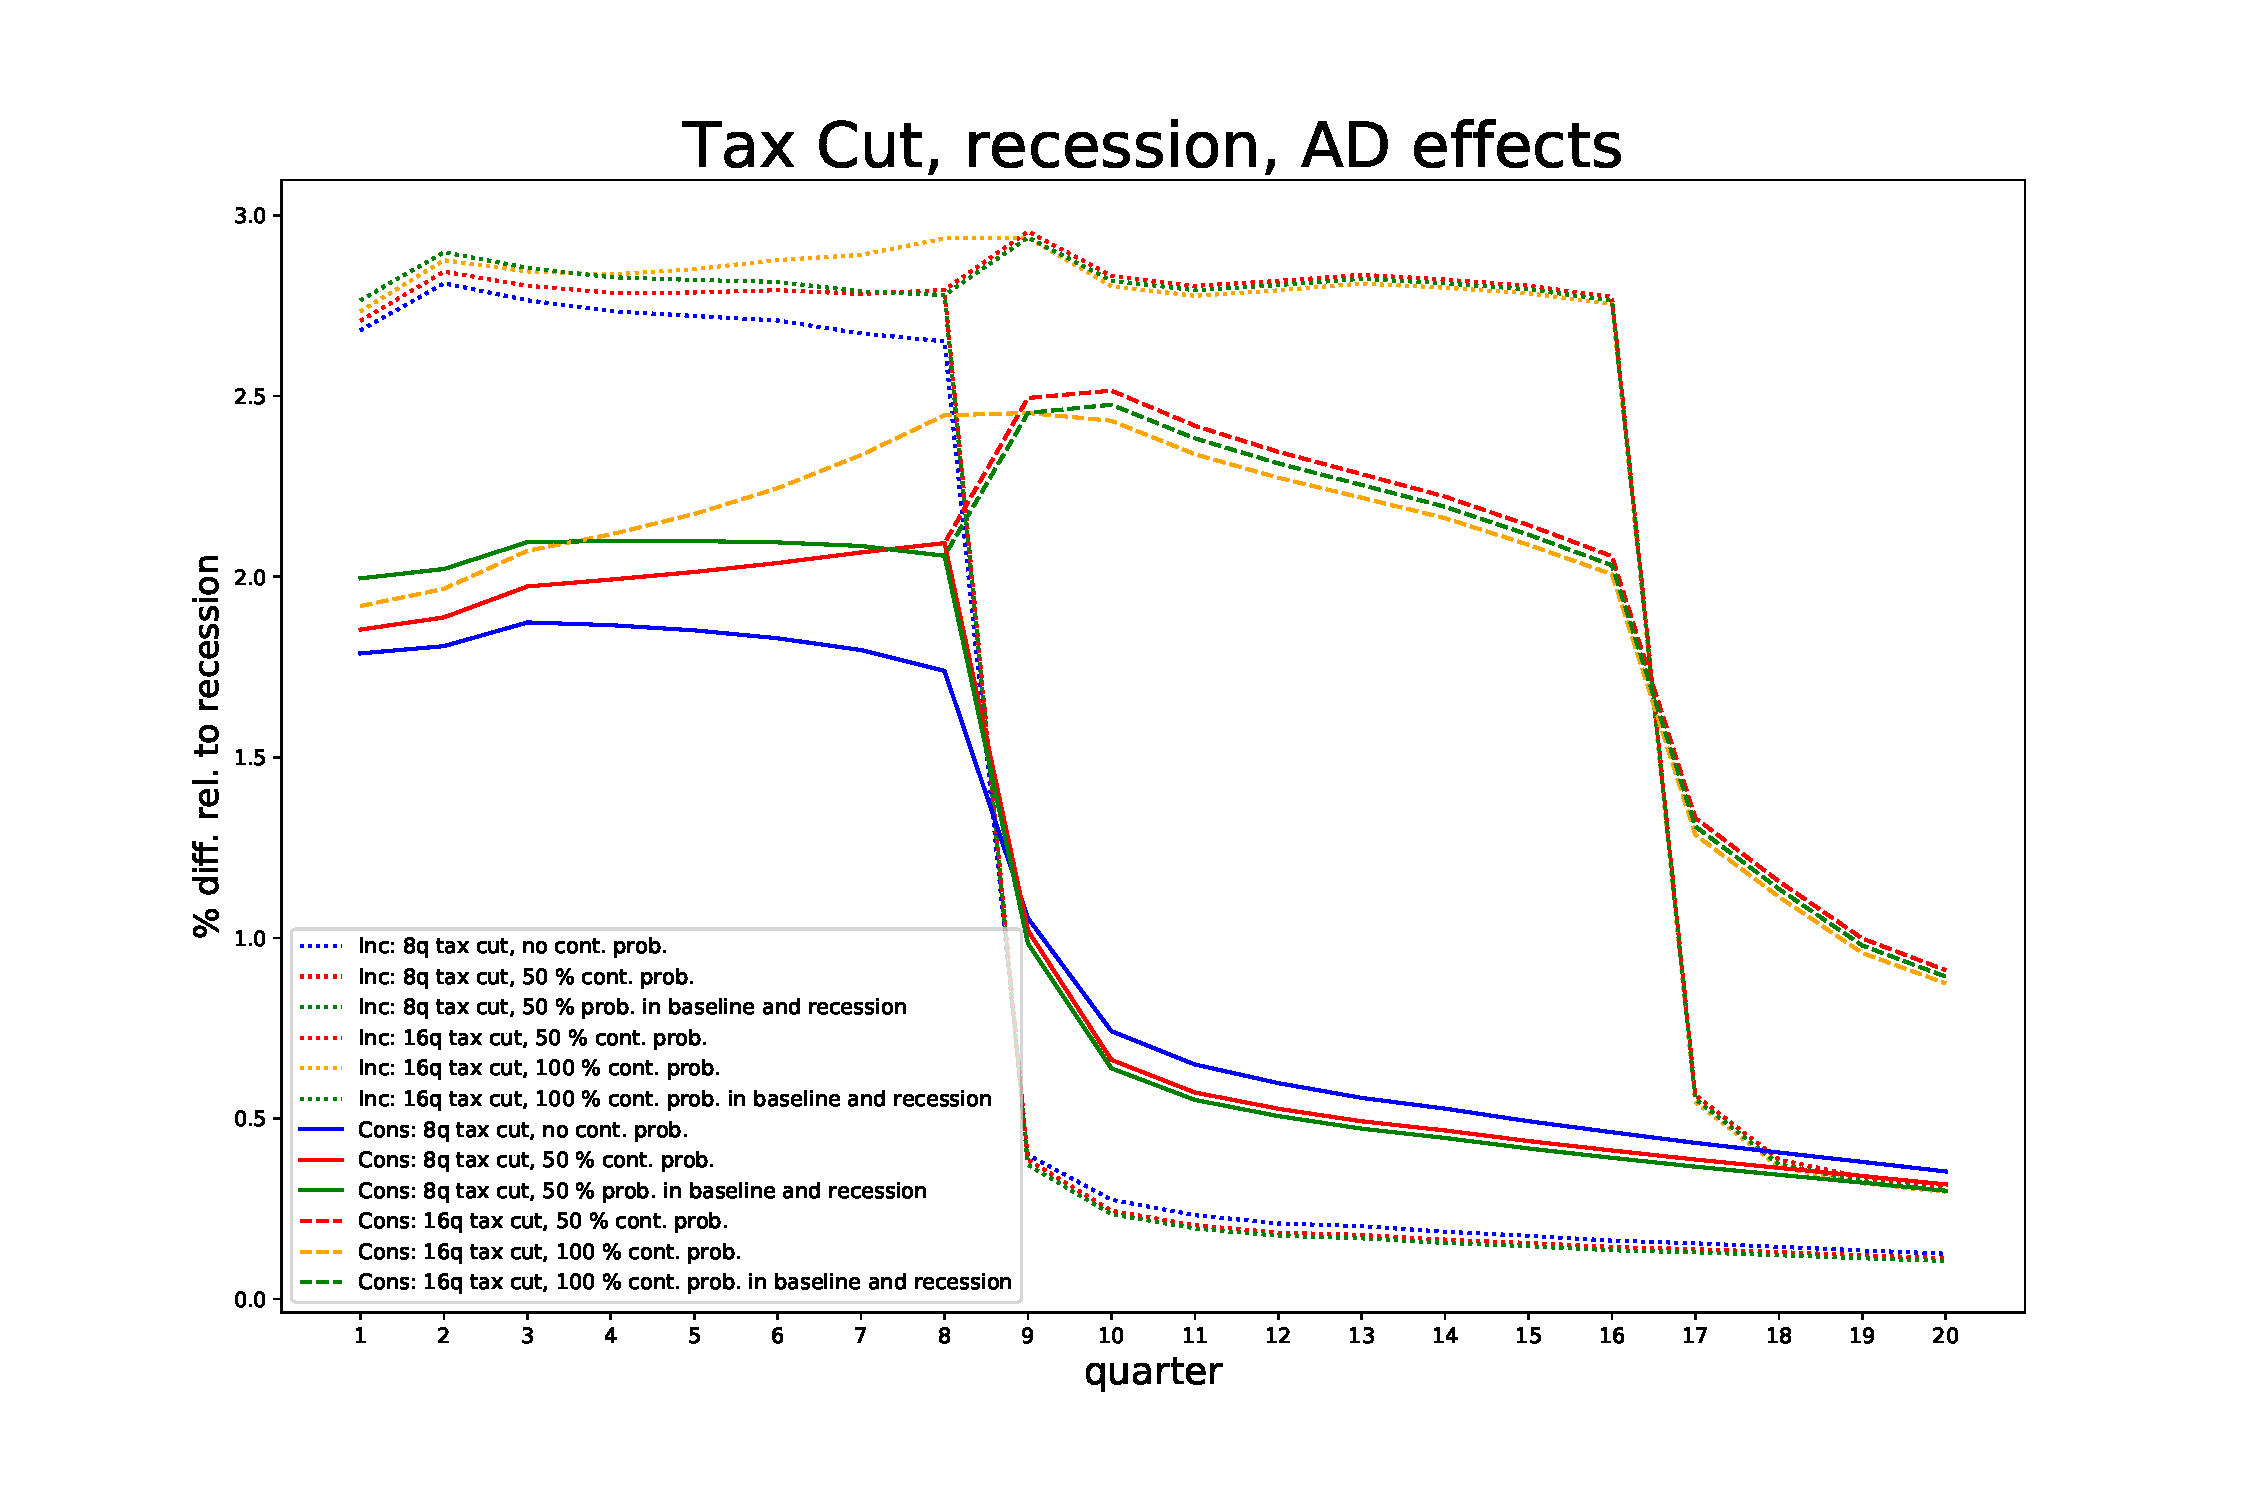
\includegraphics[width=1\linewidth]{../Continuation_Prob_Experiments/tax_cut_recession_AD_effects}
	\caption{}
	\label{fig:taxcutrecessionadeffects}
\end{figure}
	
	
	
	
	
\FloatBarrier
\section{Update - February 10th 2021}	


\FloatBarrier	
\subsection{Improved convergence}

\FloatBarrier
\subsection{Tax cut}

\begin{figure}
	\centering
	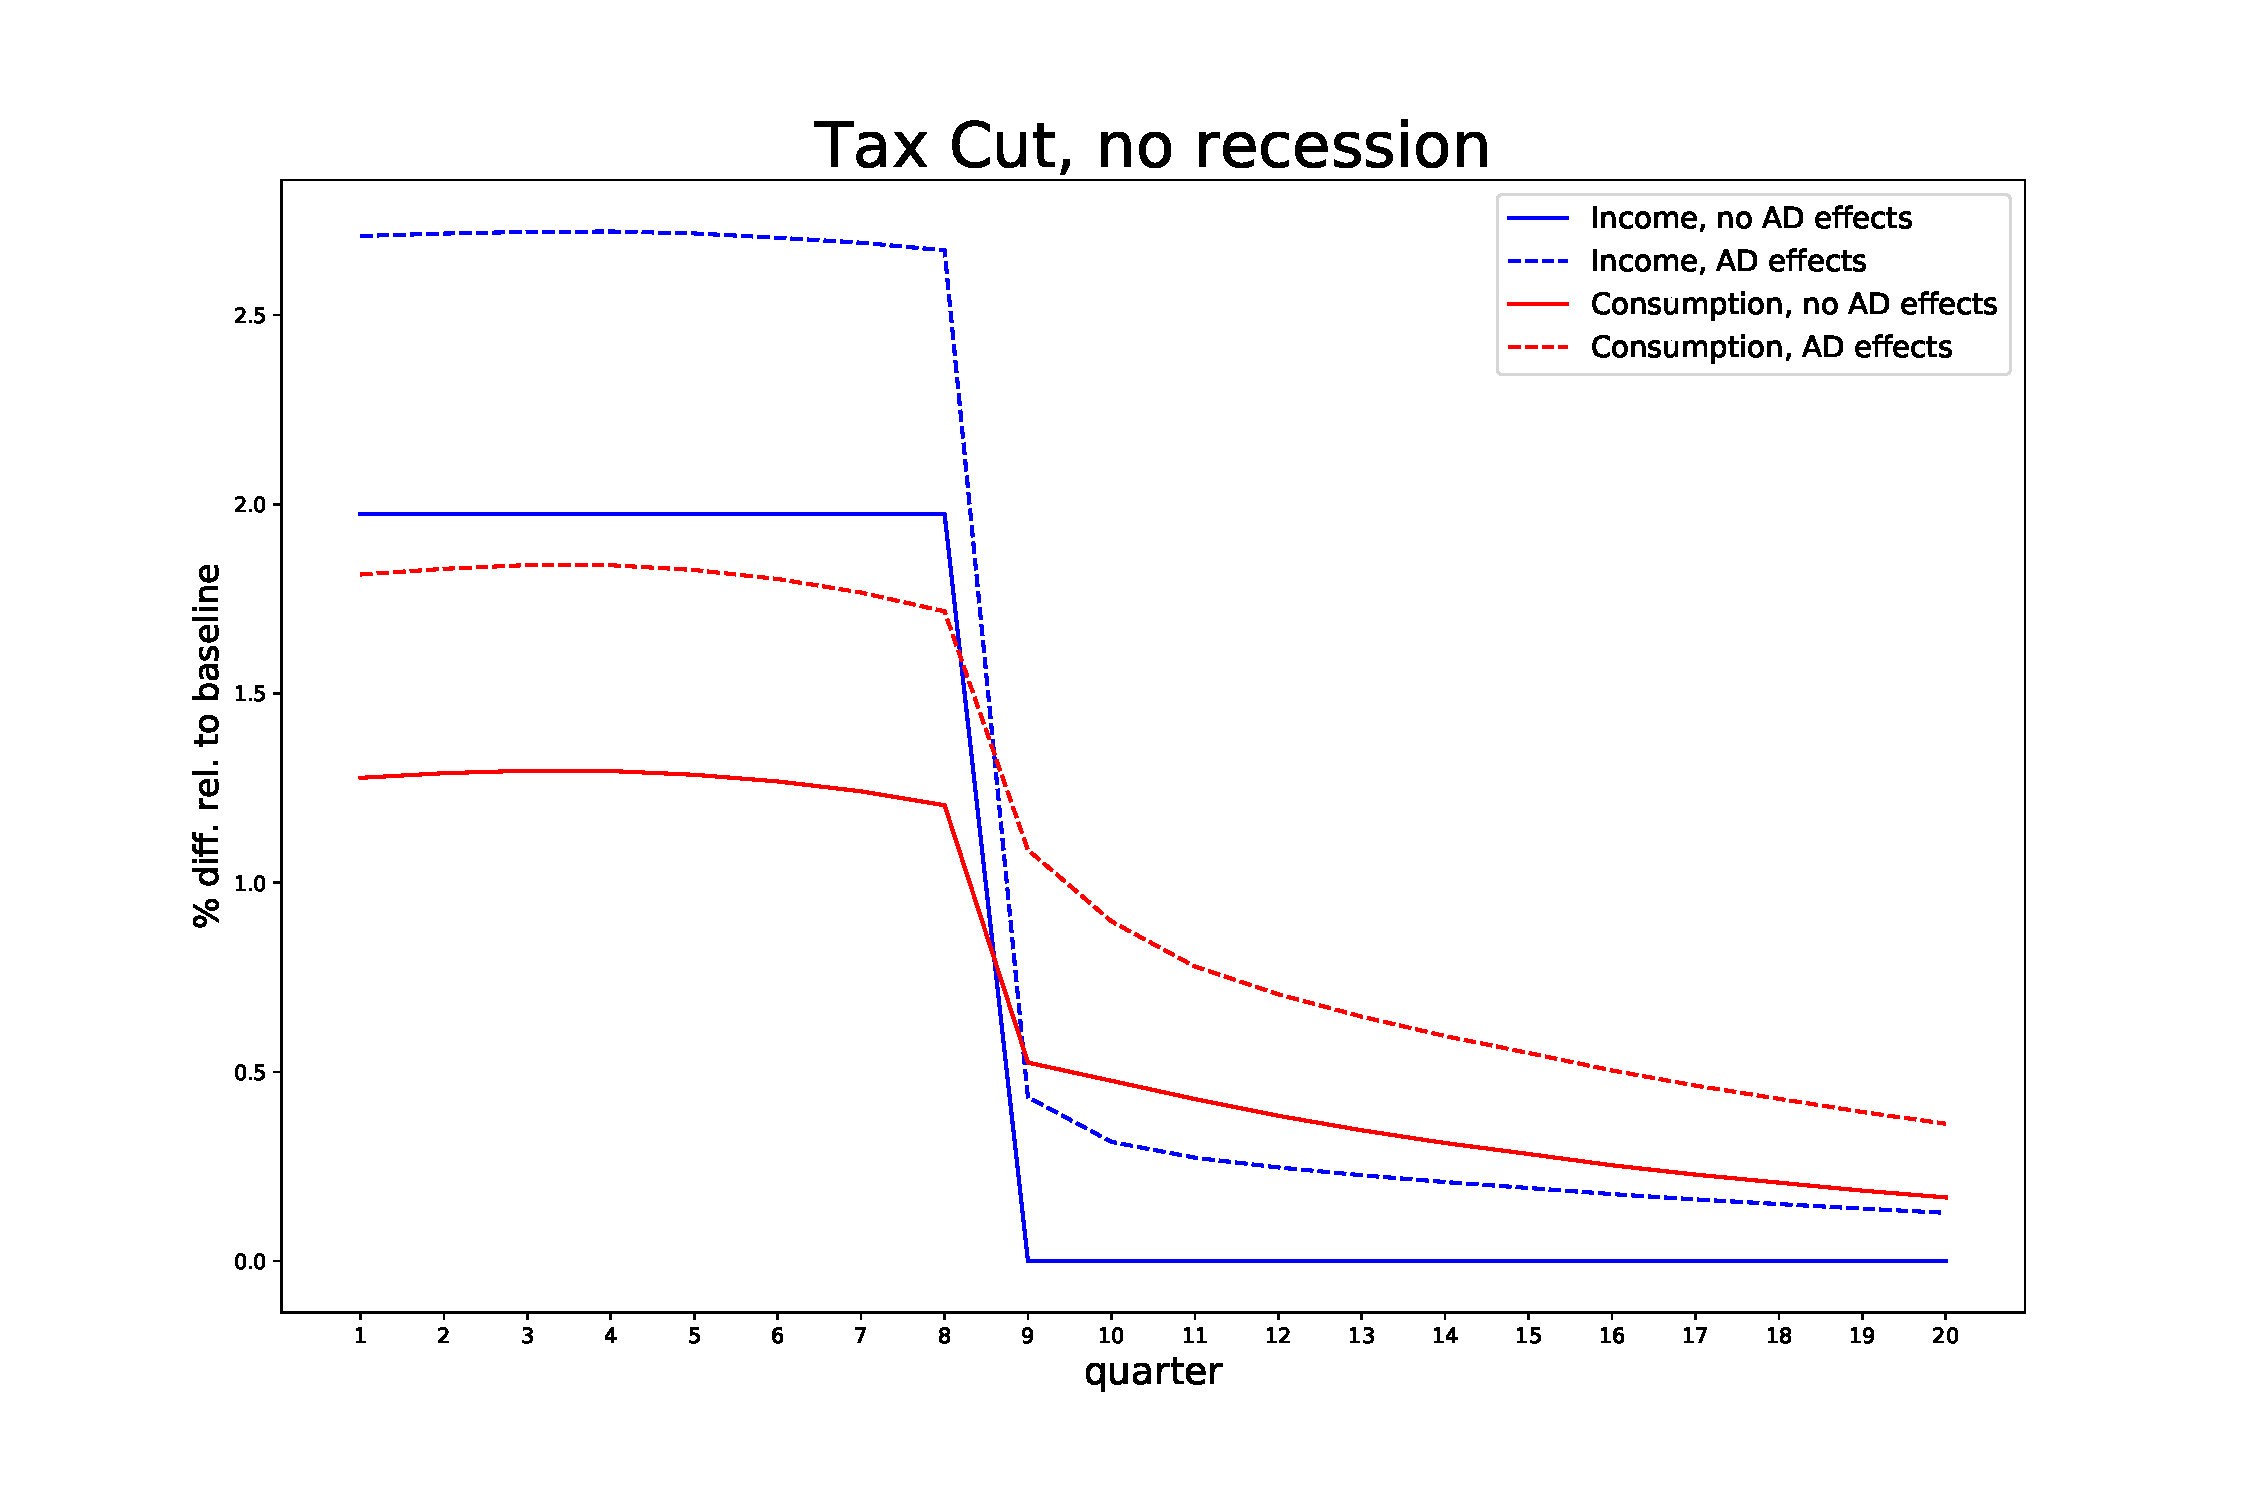
\includegraphics[width=\linewidth]{../full_run/tax_cut}
	\caption{}
	\label{fig:taxcut}
\end{figure}
\begin{figure}
	\centering
	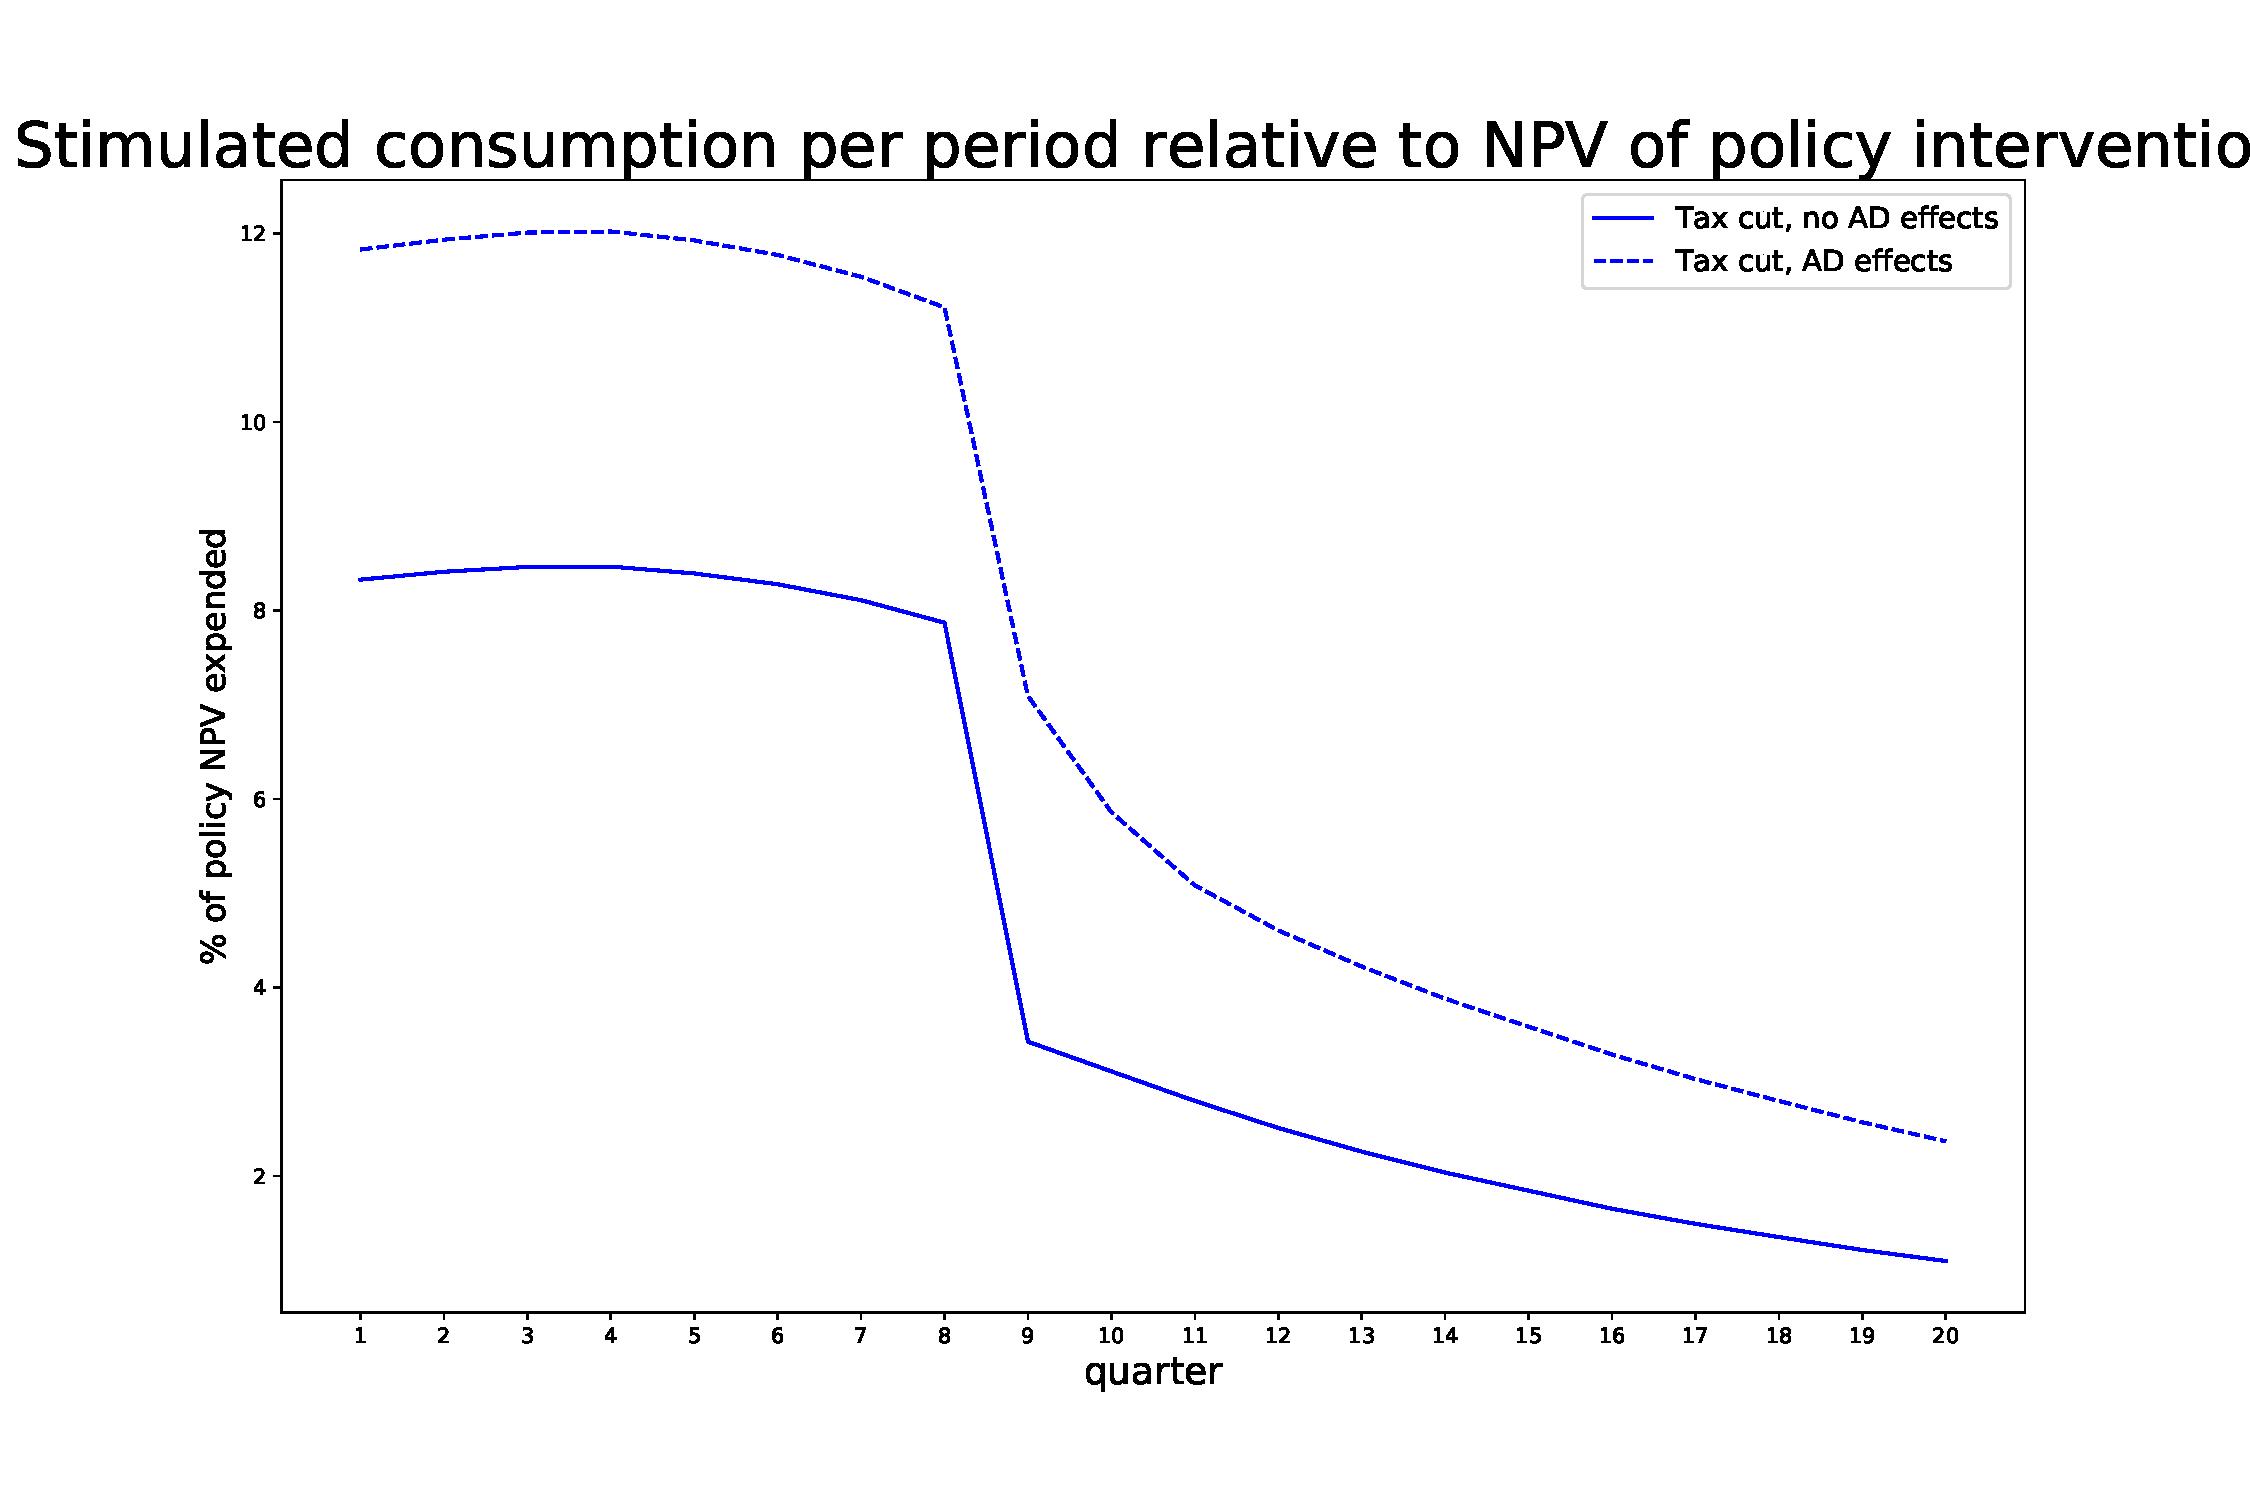
\includegraphics[width=\linewidth]{../full_run/stimulated-consumption_TaxCut}
	\caption{}
	\label{fig:stimulated-consumptiontaxcut}
\end{figure}


\begin{itemize}
	\item We consider a payroll tax cut by 2 pp for 8q (deterministic length)
	\item See Figure \ref{fig:taxcut}
	\subitem The tax increases income and consequently pushes up consumption
	\subitem The drop in consumption in 9q is due to the fact that the splurge is applied to income in excess of the baseline income, which drops to zero after the tax cut is reversed. Consumption spending remains elevated for some time after the tax cut due to built up savings. 
	\subitem With aggregate demand effects, the effect on consumption is larger as the increased consumption reinforces consumption through higher income due to higher TFP	
\end{itemize}

\FloatBarrier
\subsubsection{Recession}

\begin{figure}
	\centering
	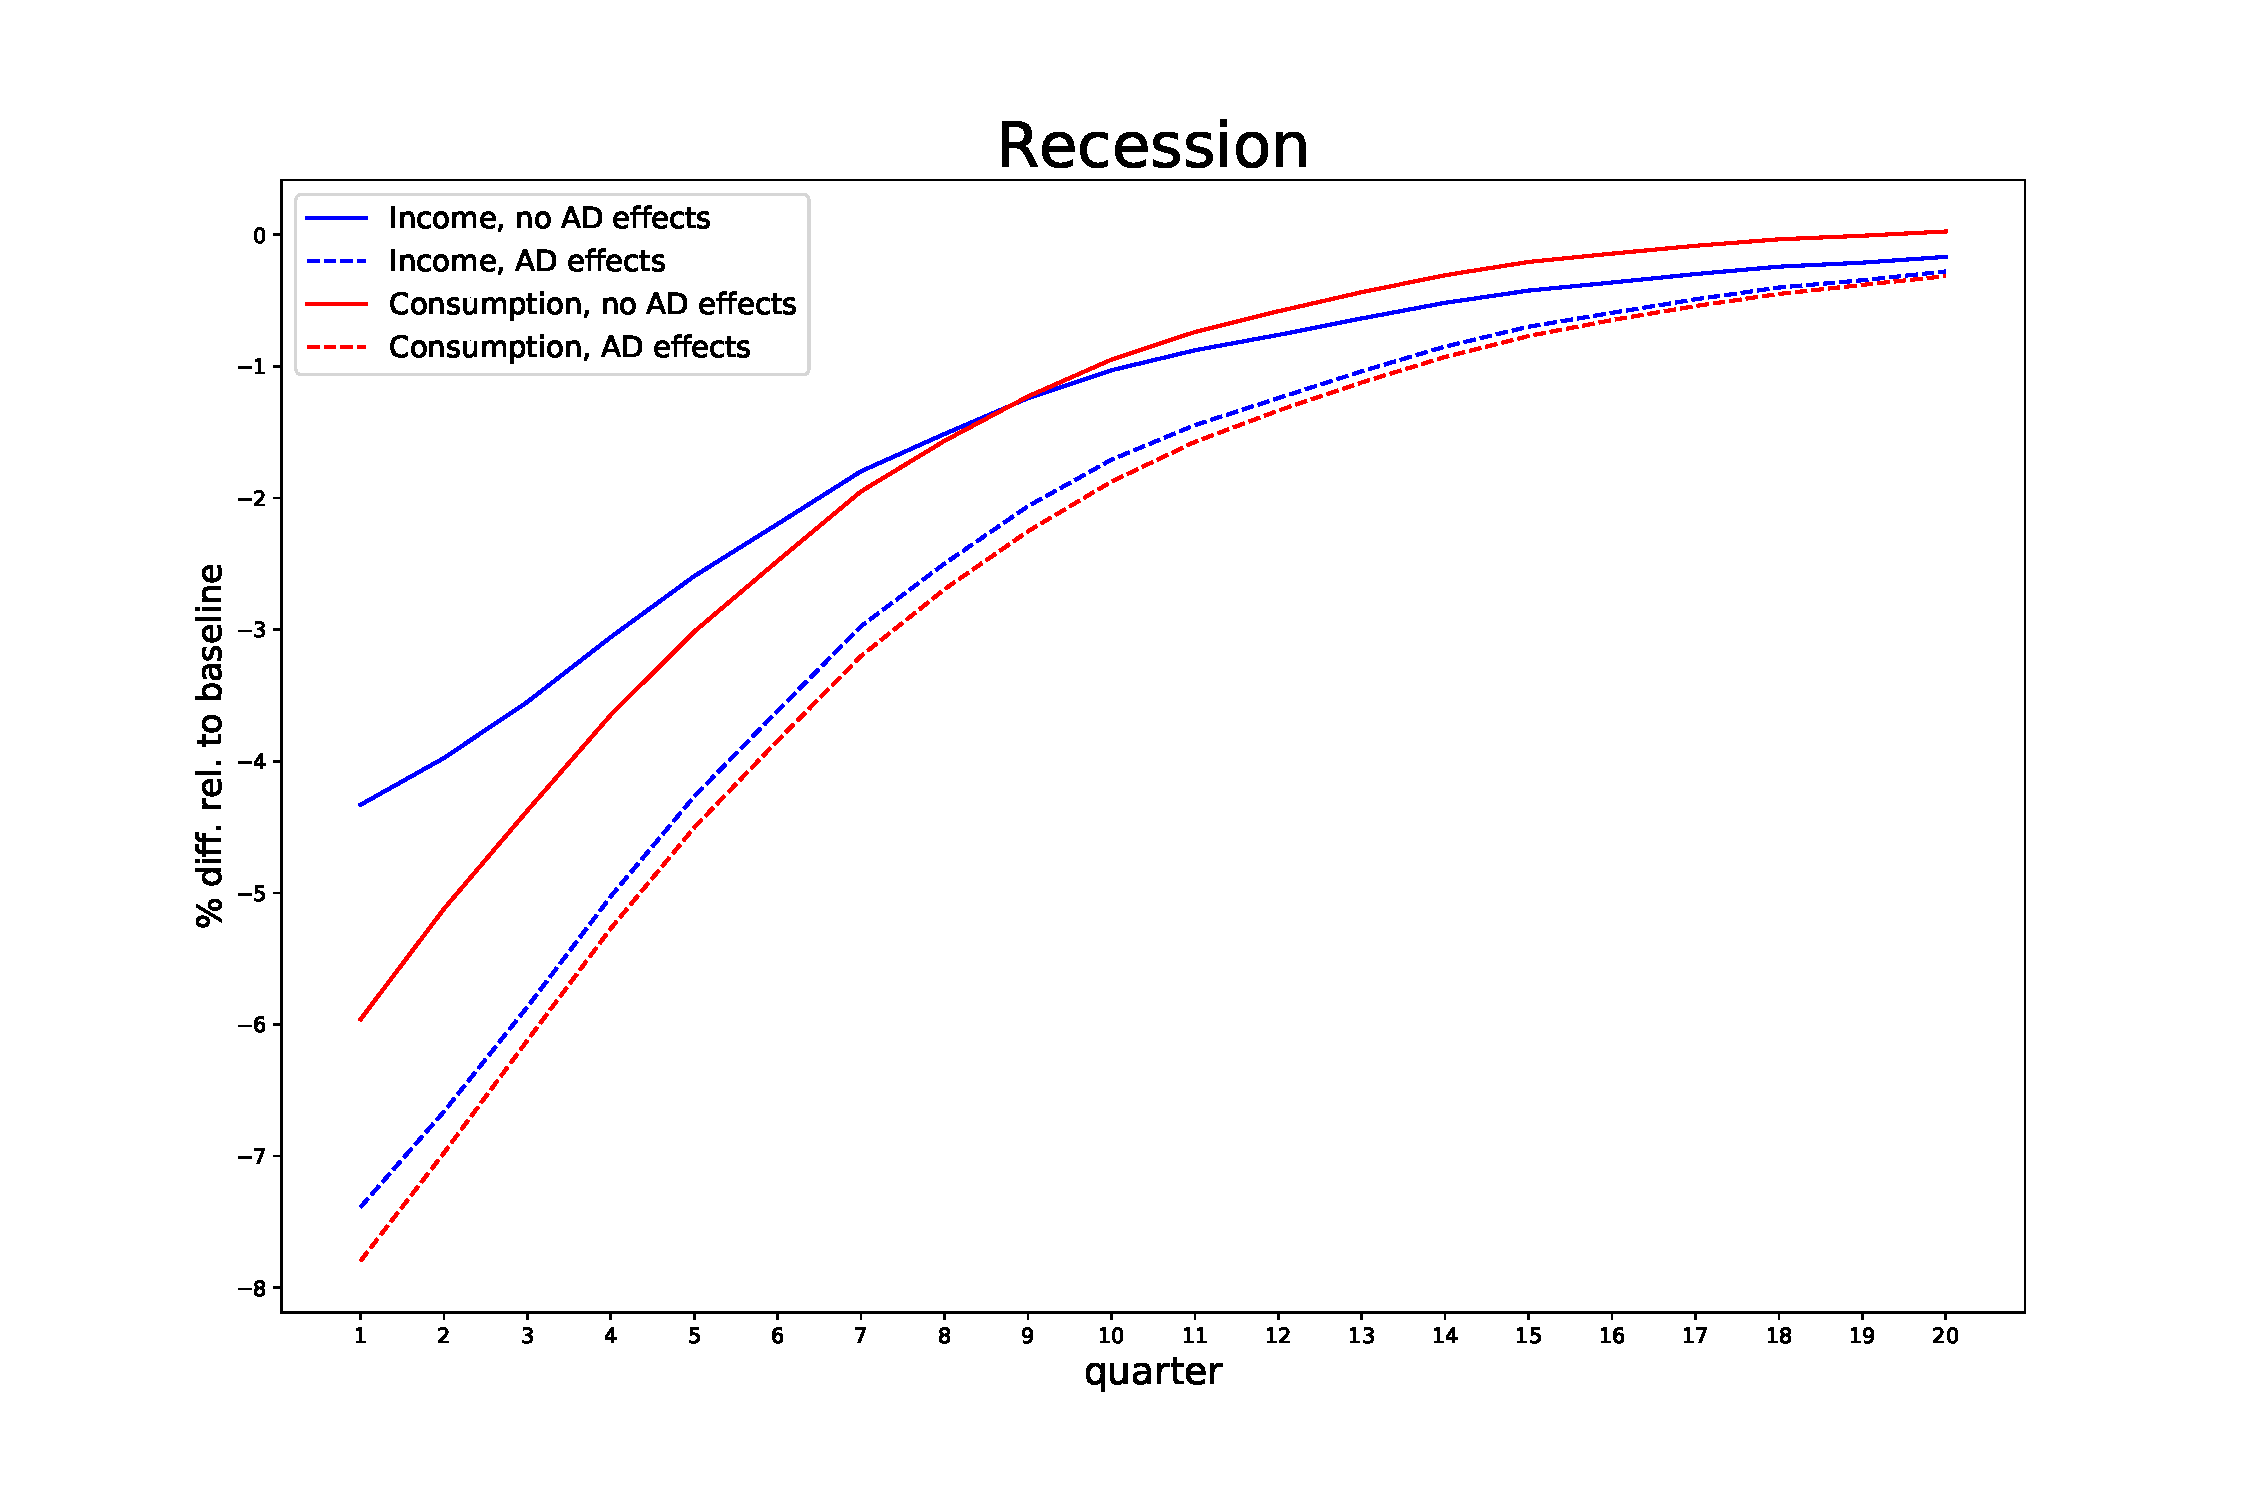
\includegraphics[width=\linewidth]{../full_run/recession}
	\caption{}
	\label{fig:recession}
\end{figure}


\begin{itemize}
	\item We consider a recession with an expected length of 6 quarters, see Figure \ref{fig:recession}
	\item In a recession the unemployment rate increases to 10 \% and lasts on average 4 quarters (as opposed to 5\% / 1.5 q in normal times)
	\item The recession depresses aggregate income due to loss of labor income, only partly compensated by unemployment benefits (lasting 2 q, replacing 30 \% of income)
	\item Consumption falls as income is lower.
	\item The recession is deeper when productivity depends on aggregate demand.
\end{itemize}




\FloatBarrier
\subsection{Tax cut during recession}


\begin{figure}
	\centering
	\begin{subfigure}[b]{\textwidth}
		\centering
		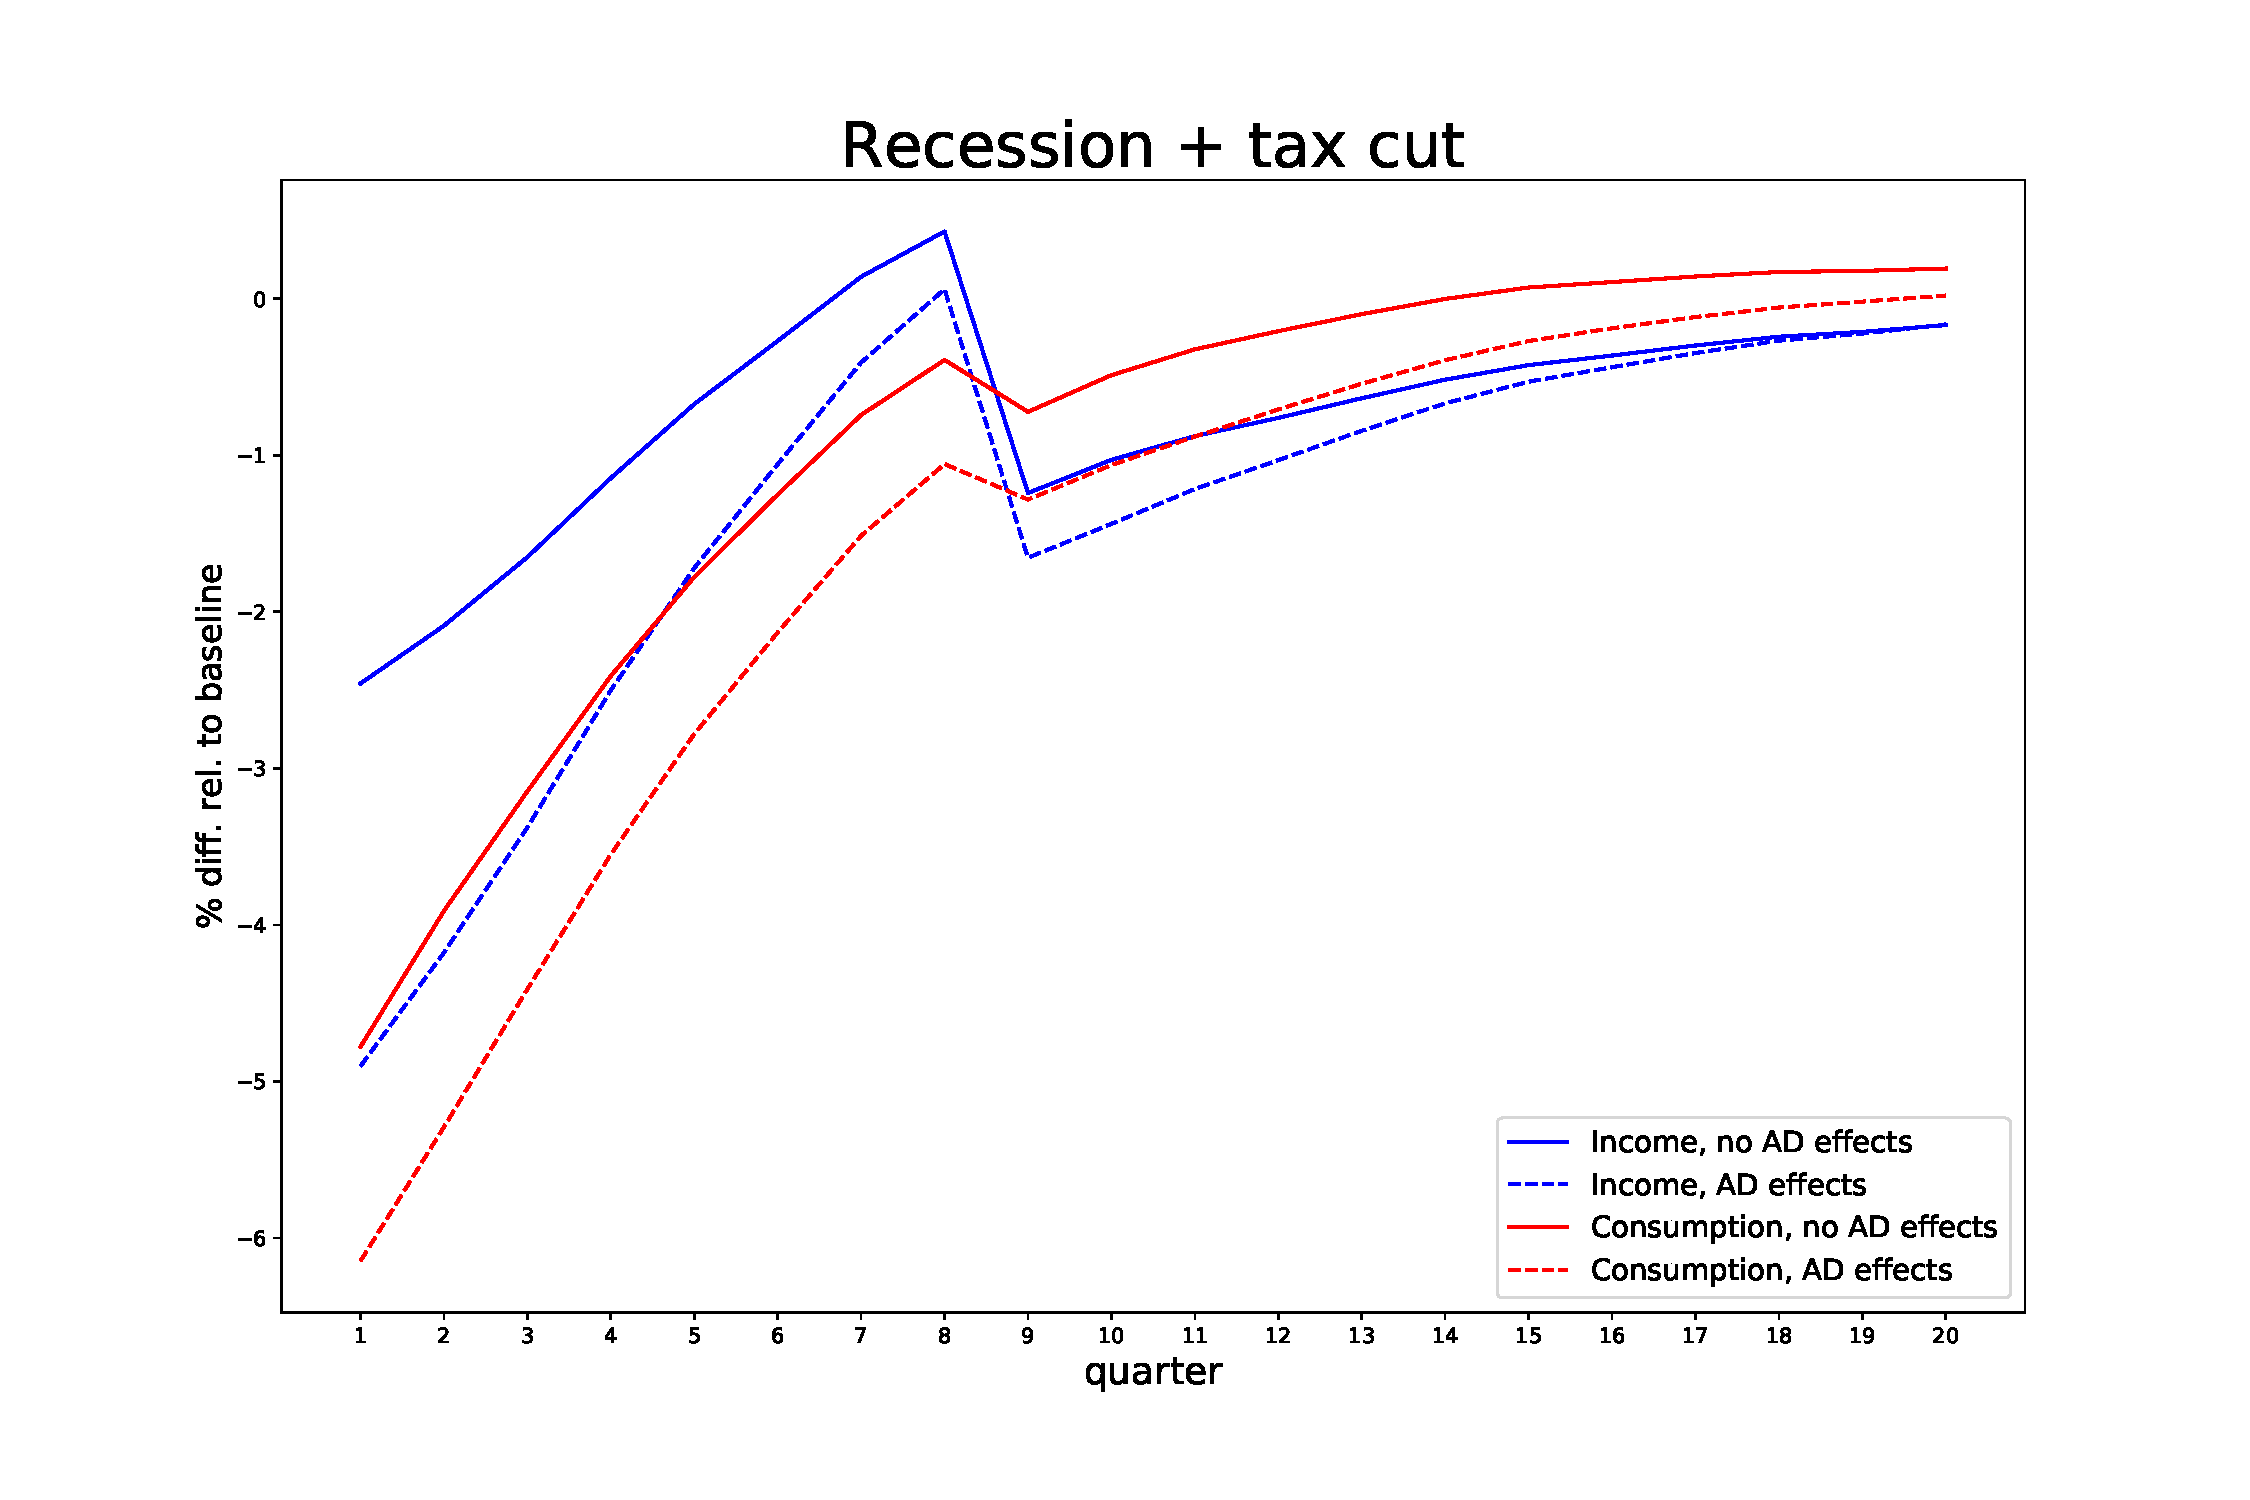
\includegraphics[width=\linewidth]{../full_run/recession_taxcut_relbaseline}
		\caption{rel. to baseline}
		\label{fig:recessiontaxcutrelbaseline}
	\end{subfigure}\\
	\hfill
	\begin{subfigure}[b]{\textwidth}
	\centering
	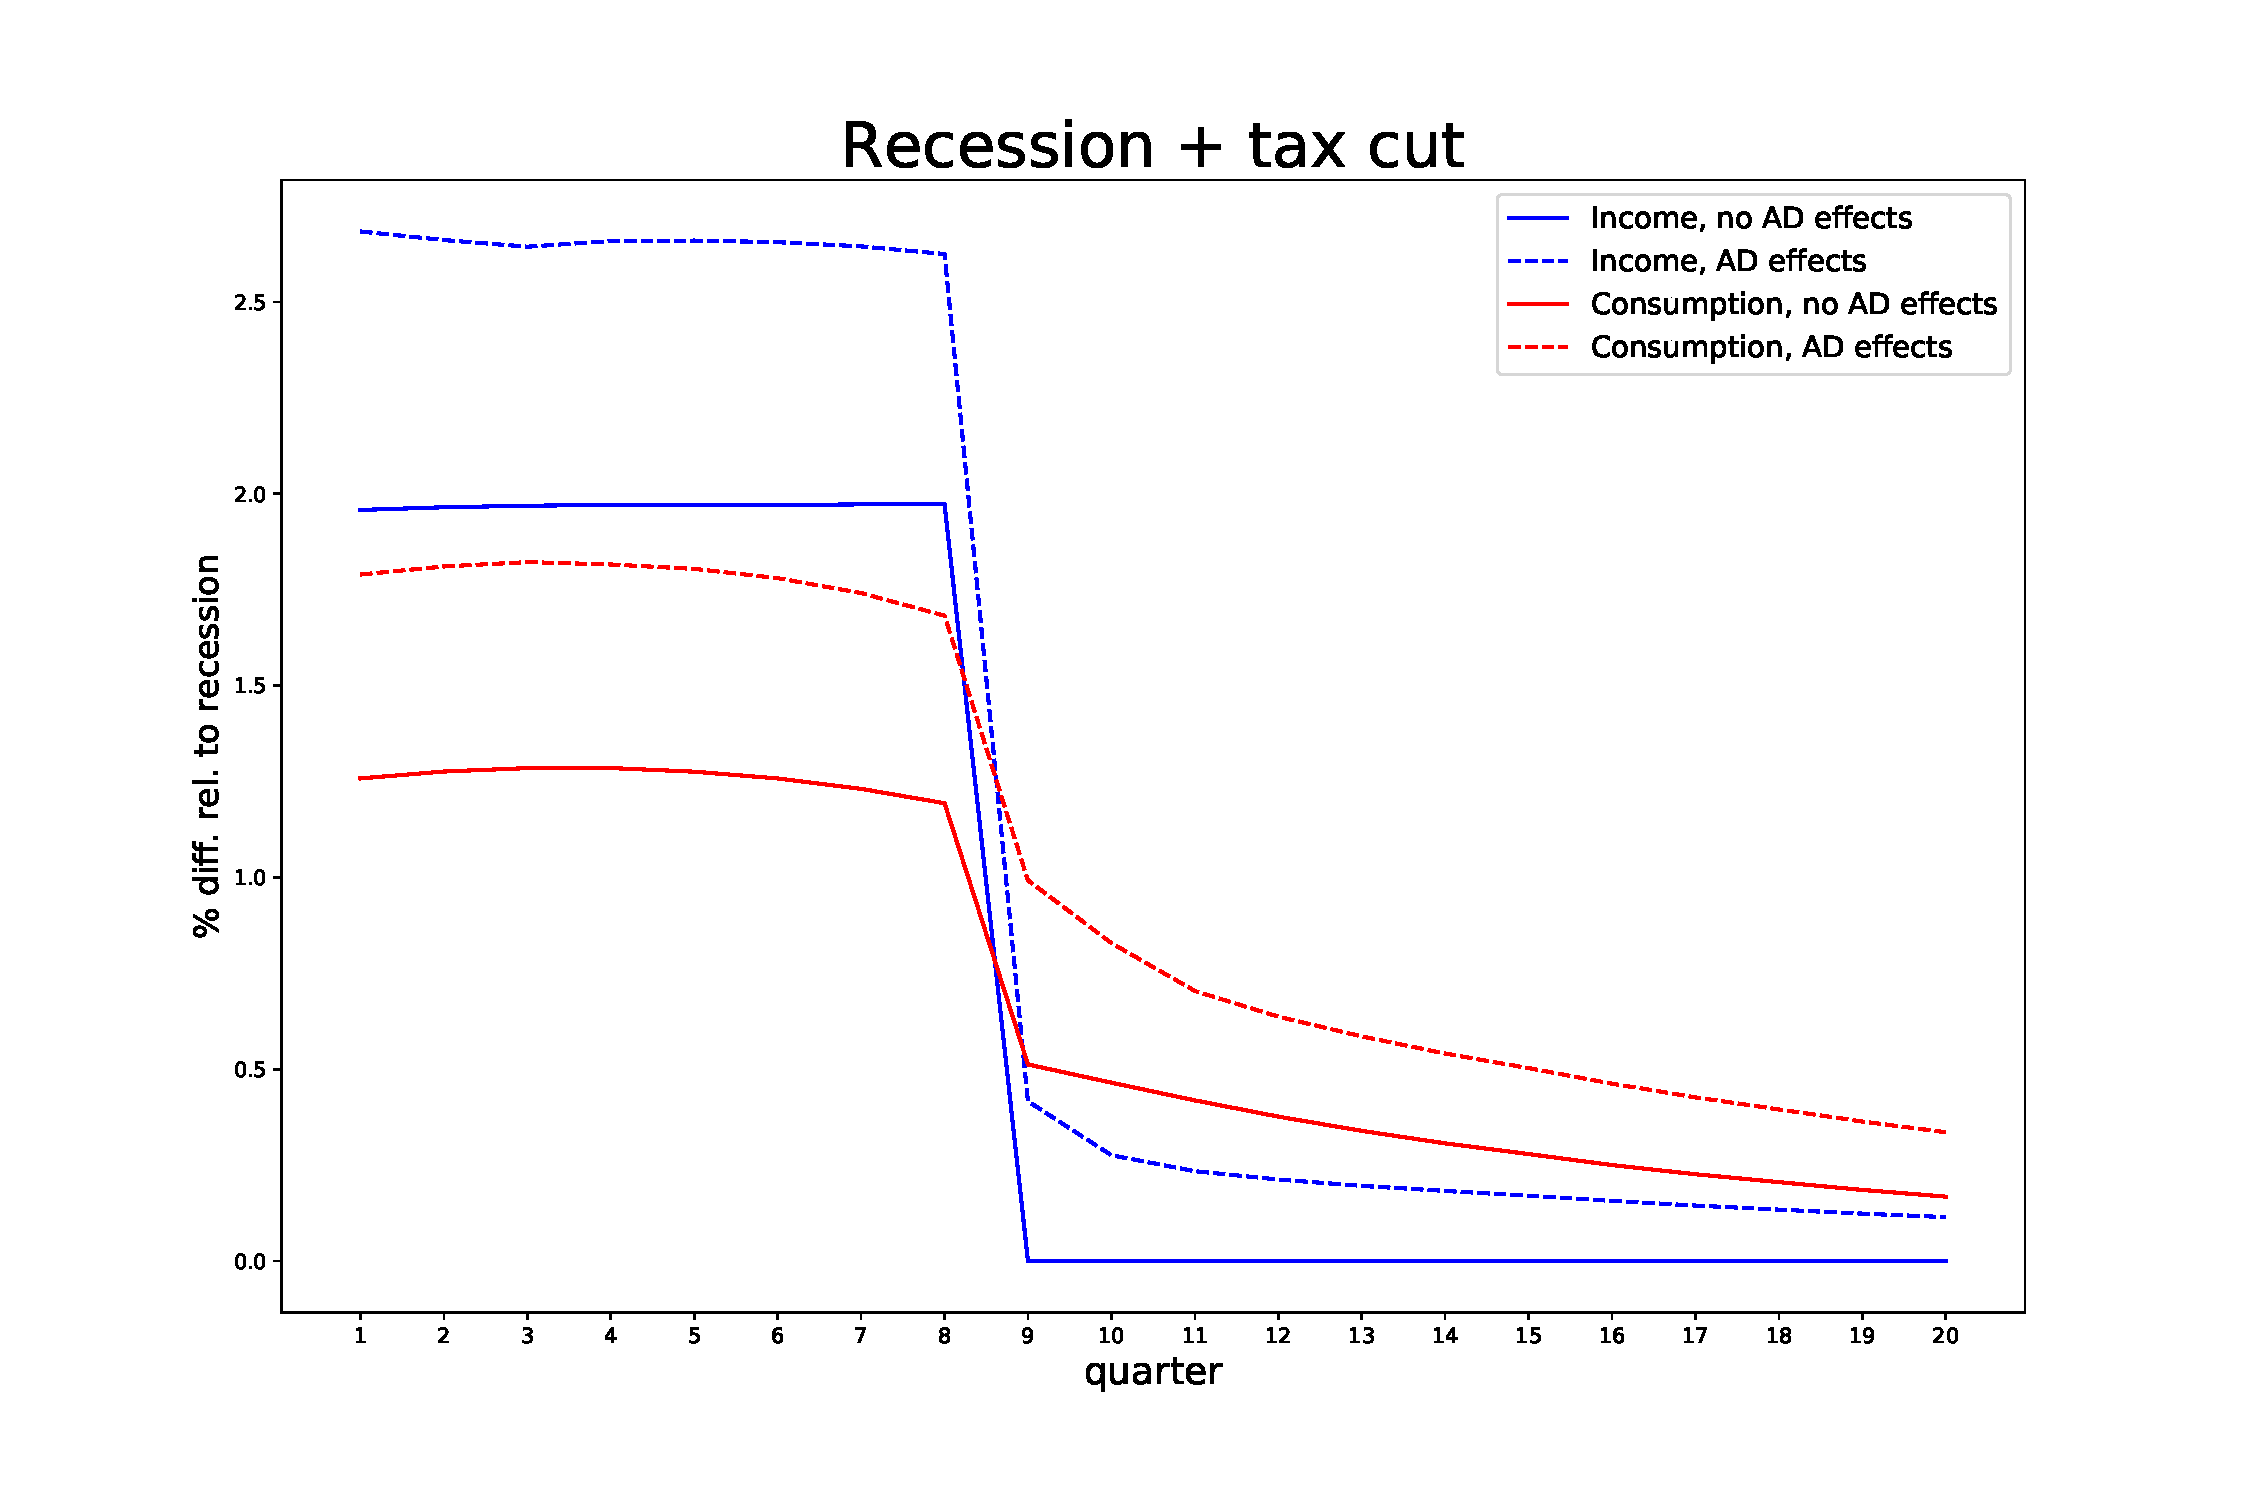
\includegraphics[width=\linewidth]{../full_run/recession_taxcut_relrecession}
	\caption{rel. to recession}
	\label{fig:recessiontaxcutrelrecession}
	\end{subfigure}
\end{figure}

\begin{figure}
	\centering
	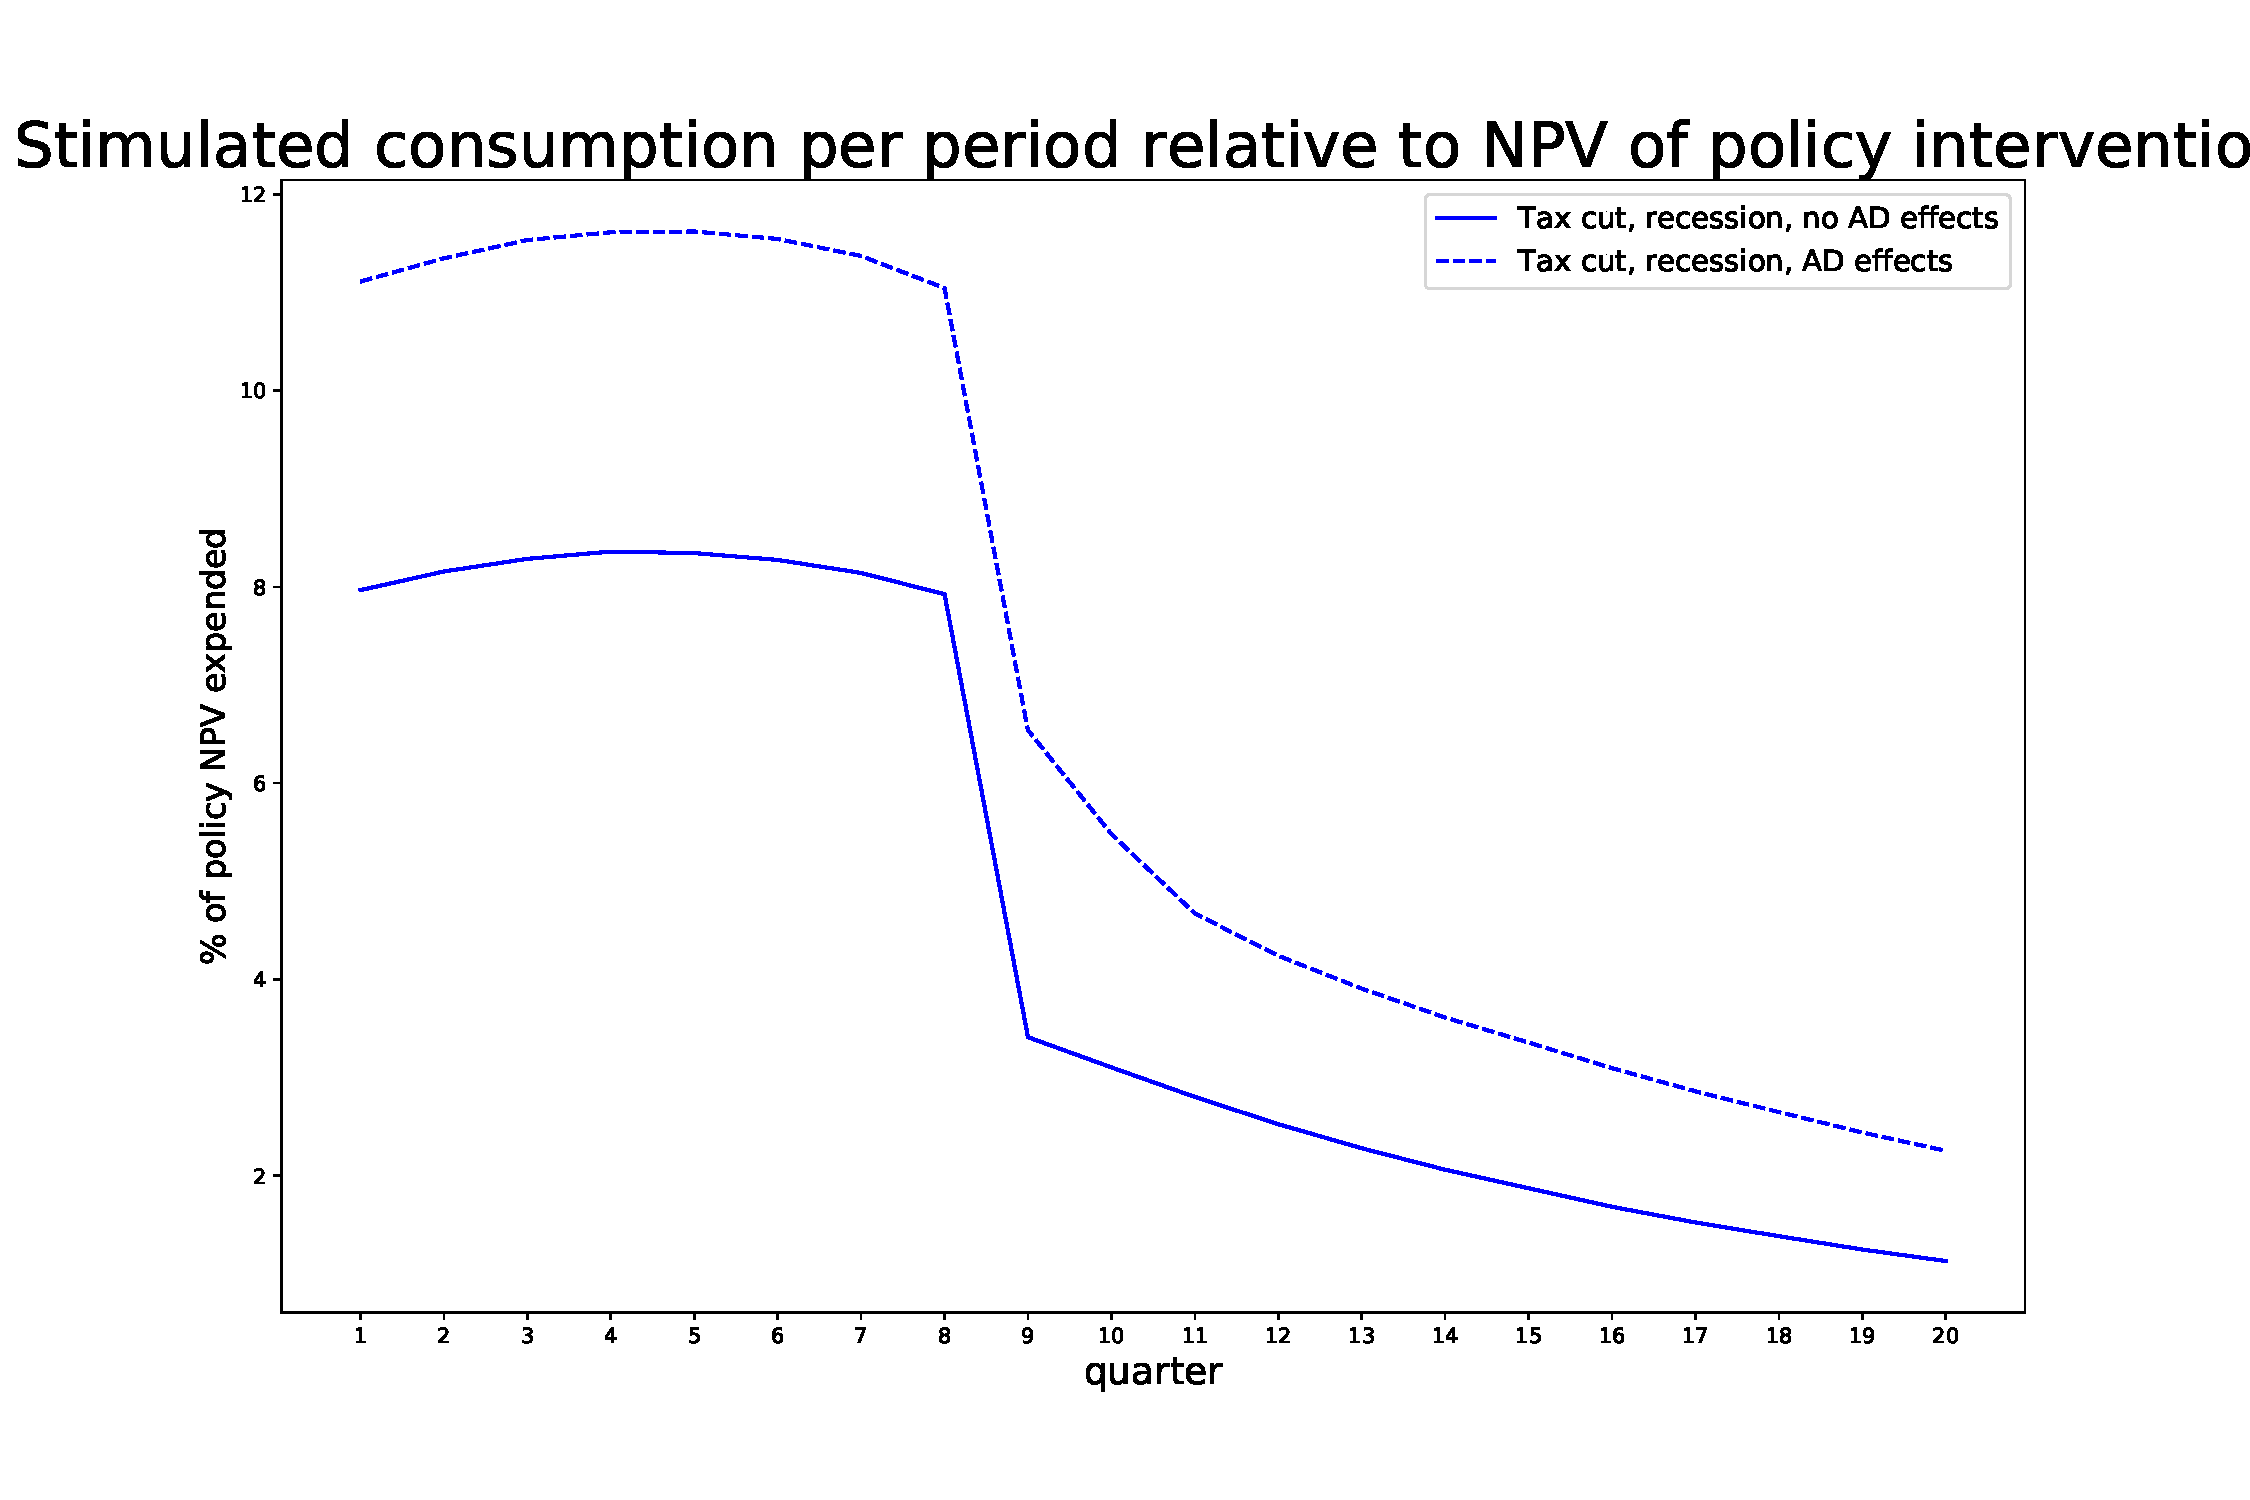
\includegraphics[width=\linewidth]{../full_run/stimulated-consumption_RecTaxCut}
	\caption{}
	\label{fig:stimulated-consumptionrectaxcut}
\end{figure}



\begin{itemize}
	\item We consider a payroll tax cut by 2 pp for 8q (deterministic length) during a recession with an expected length of 6q 
	\item Additional income / consumption relative to the baseline (see figure \ref{fig:taxcutrecession}) and to recession scenario (see figure \ref{fig:taxcutrecession2})
	\item When AD effects are switched off we obtain a similar result as in the baseline. However, note, that as the recession disappears, the additional income by the tax cut increases as more people are employed
	\item This upward trend in the effect of the tax cut is much more pronounced when considering AD effects. This is because very low consumption at the beginnning of the recession sets a much steeper recovery path.
	\item Not clear why consumption first drops (numerical error?)
\end{itemize}


	
\FloatBarrier	
\subsection{Deterministic length of the payroll tax cut vs. probability of continuation}

We compare a payroll tax cut (of 2 percentage points) when the length of the payroll tax cut policy is deterministic and set to eight quarters vs. when there is a 50\% chance (of which everyone is aware) of an continuation of the initial eight quarter of payroll tax cut by another eight quarters (and so on). We do so with and without aggregate demand (AD) effects.

\begin{itemize}
	\item Figure \ref{fig:taxcutnorecessionnoadeffects} shows the payroll tax cut without AD effects
	\item Income increases for either 8 or 16 q depending on scenario
	\item Consumption during the first 8q is higher when there is a chance of continuation of the policy even if it does not materialize. If it does not materialize consumption in quarter 9 falls below the level relative to the scenario where continuation was excluded out in the first place, because consumption was based on the expected income.
	\item When the continuation actually occurs, agents increase consumption because actual income exceeds expected income.
\end{itemize}

\begin{figure}
	\centering
	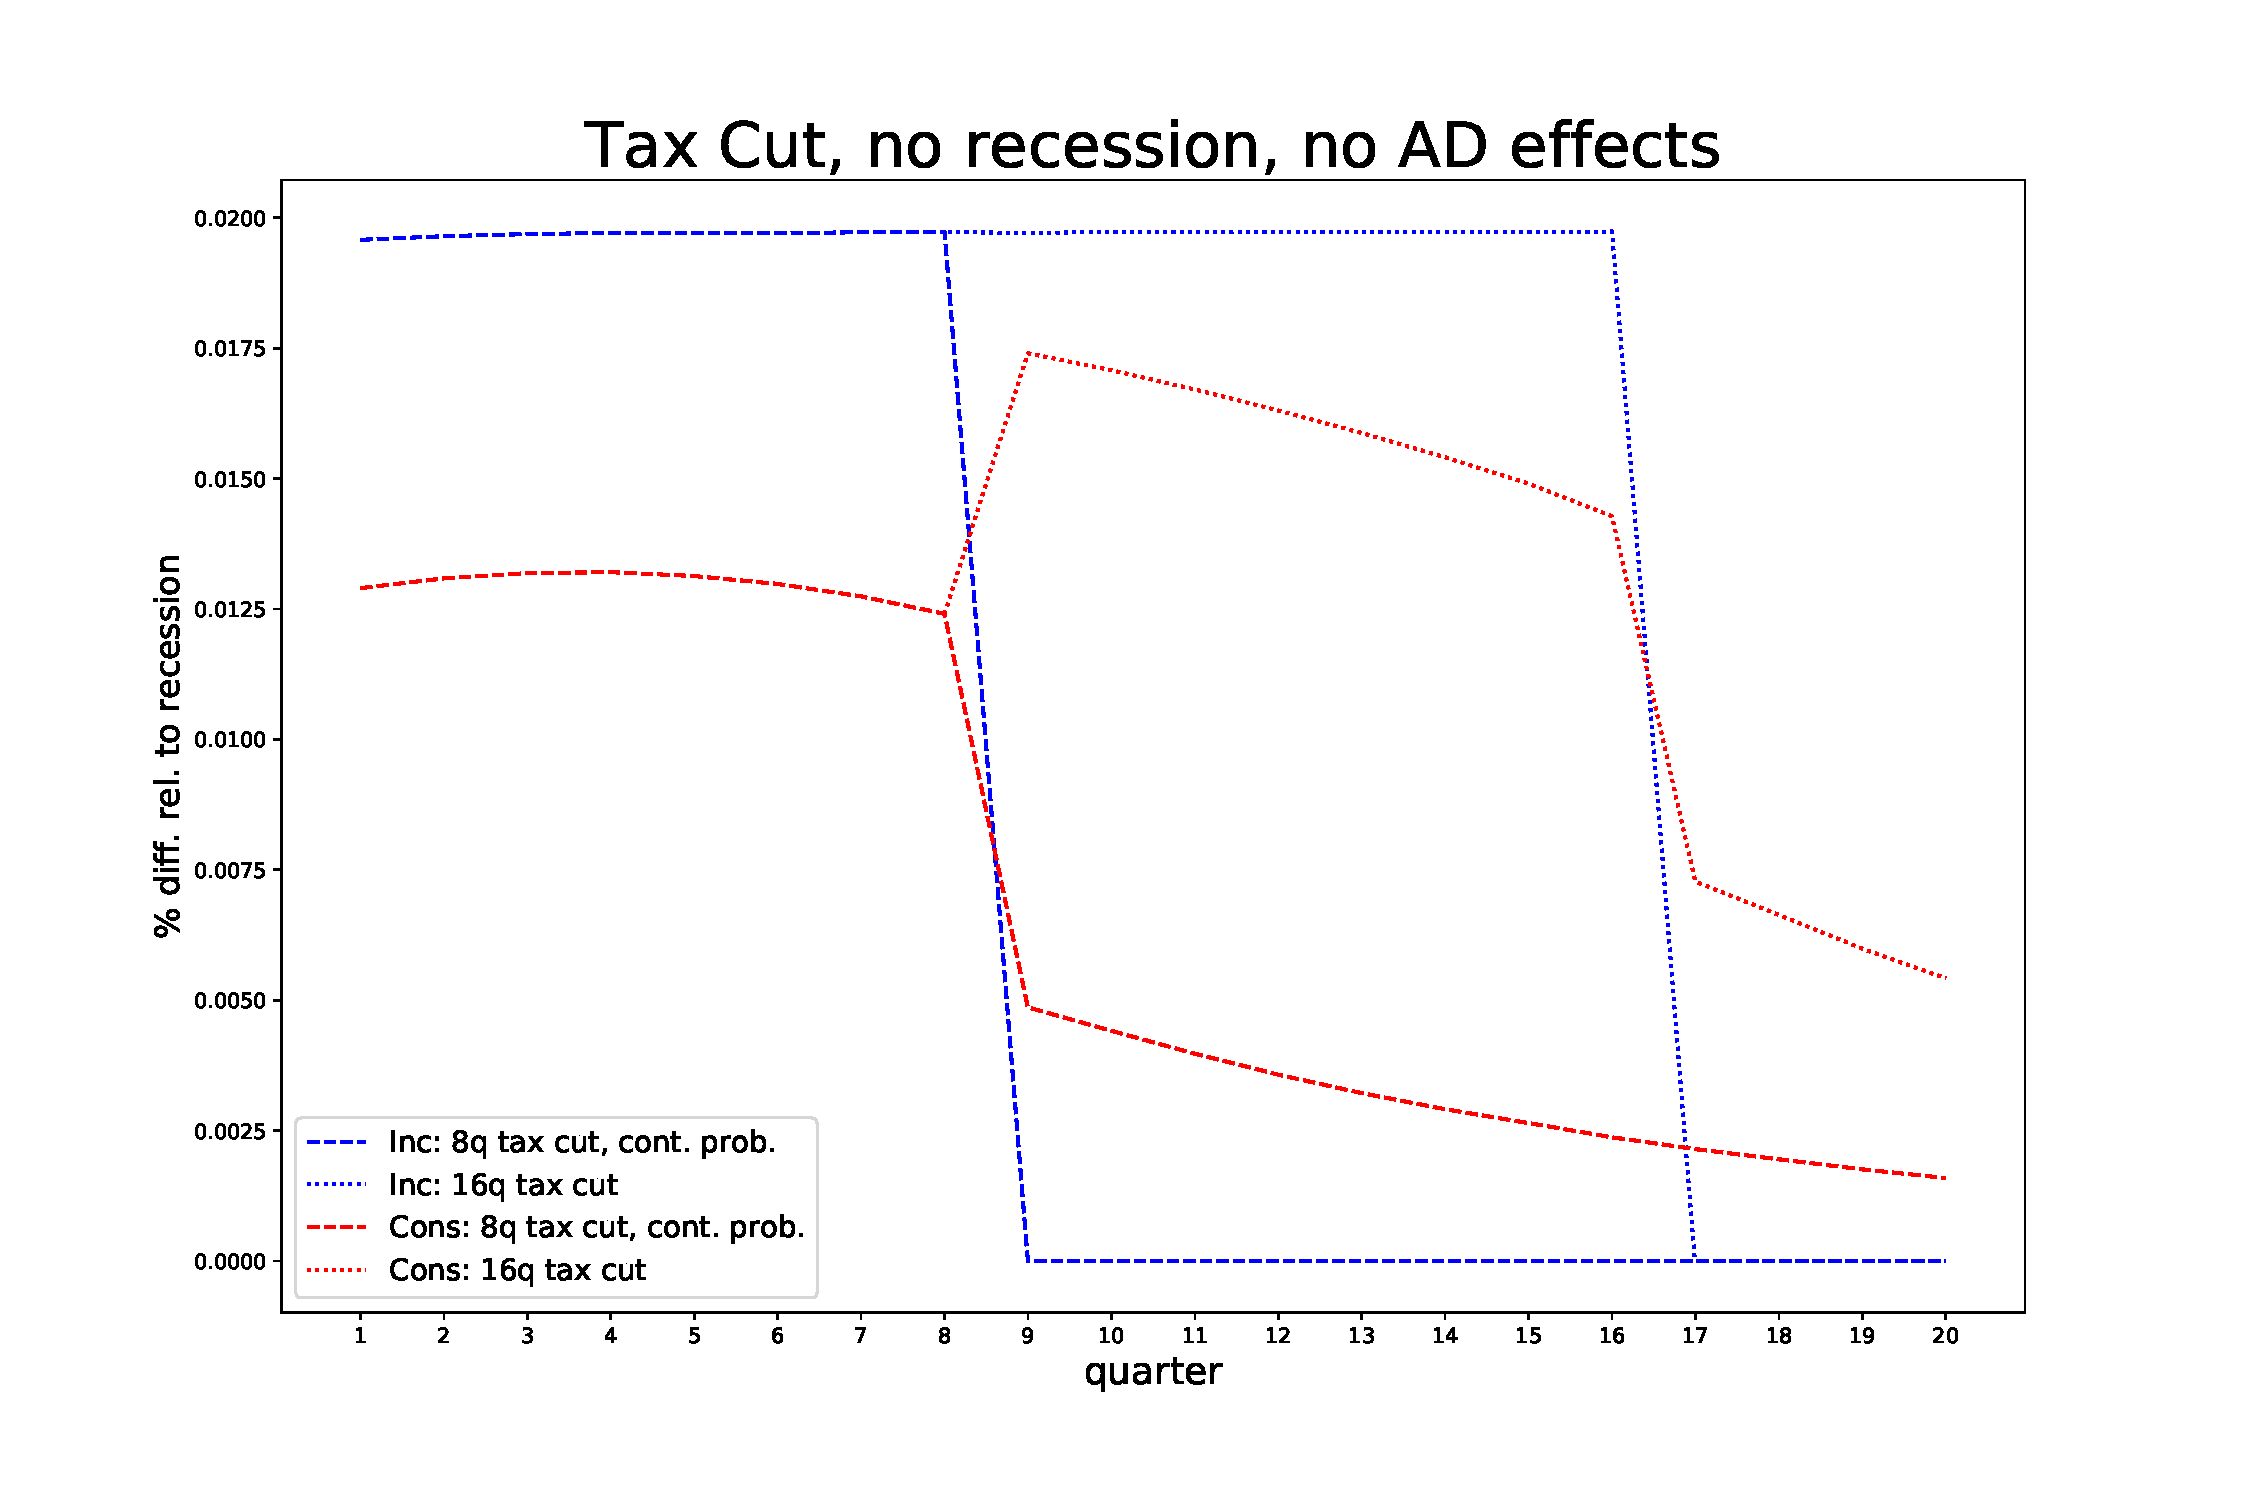
\includegraphics[width=\linewidth]{../Continuation_Prob_0/tax_cut_no_recession_no_AD_effects}
	\caption{}
	\label{fig:taxcutnorecessionnoadeffects}
\end{figure}

\begin{itemize}
	\item Figure \ref{fig:taxcutnorecessionadeffects} shows the payroll tax cut with AD effects
	\item Income increases for either 8 or 16 q depending on scenario. However, income now increase by more than 2\% percent because of AD effects, implying an additional boost to income when the continuation of the payroll tax cut is implemented.
\end{itemize}
	
\begin{figure}
	\centering
	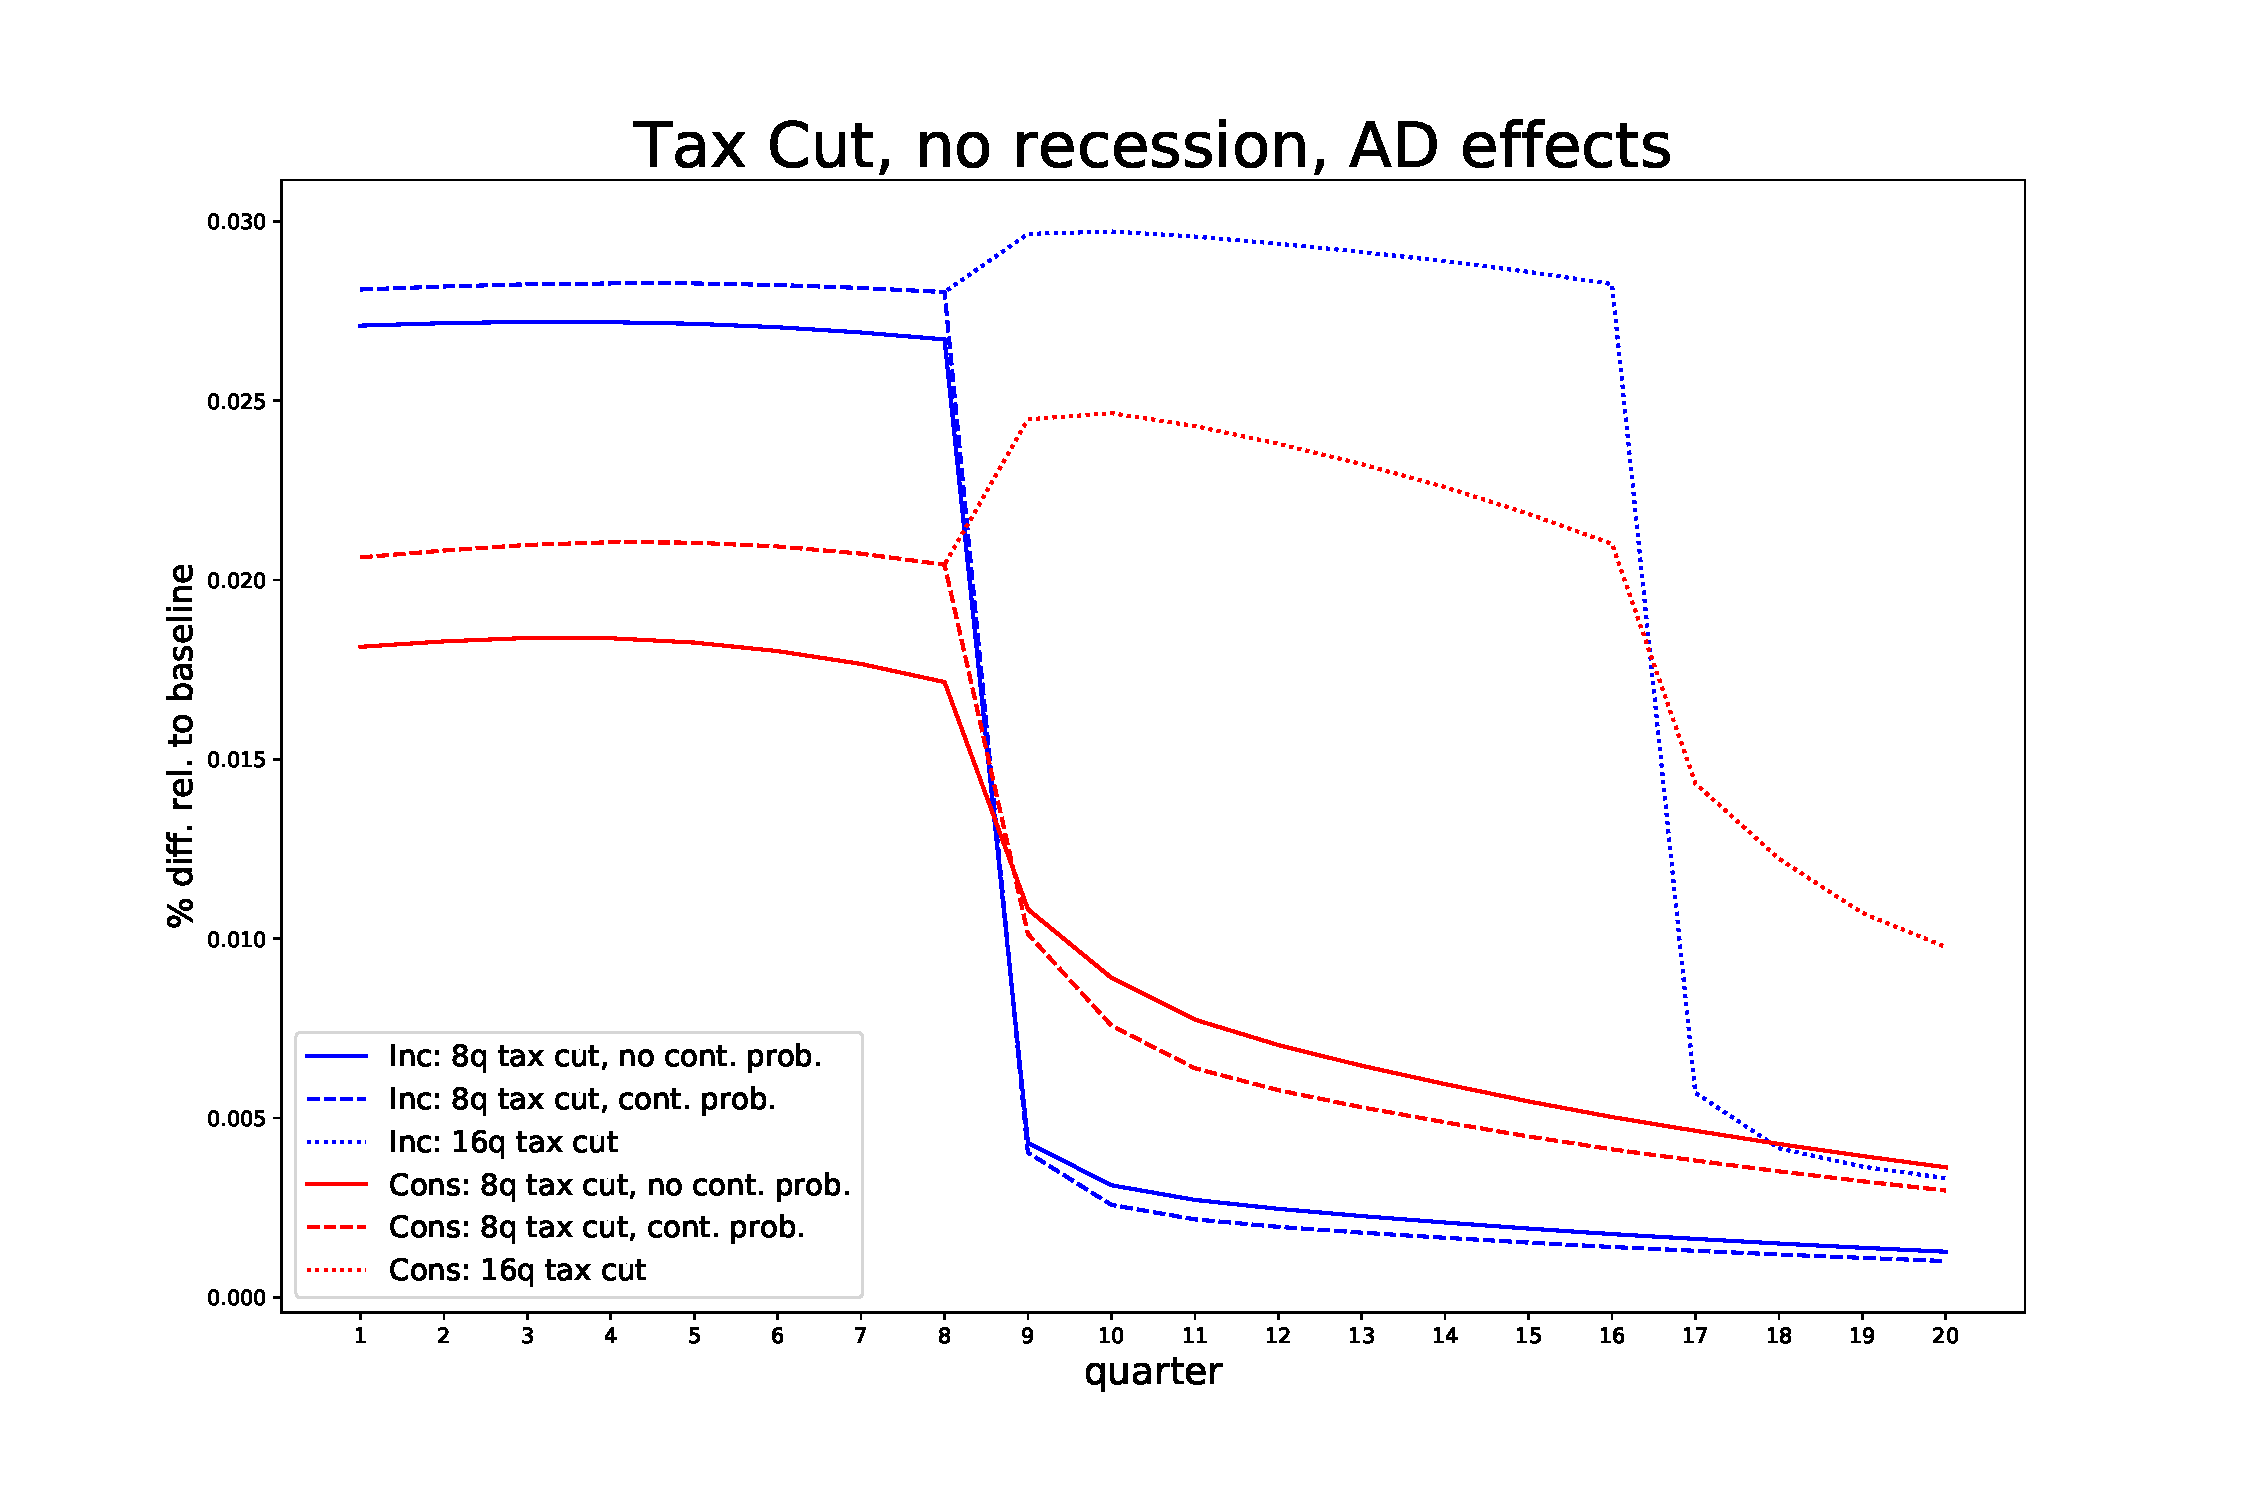
\includegraphics[width=\linewidth]{../Continuation_Prob_0/tax_cut_no_recession_AD_effects}
	\caption{}
	\label{fig:taxcutnorecessionadeffects}
\end{figure}



\FloatBarrier
\subsection{Sample size and speed of simulation}

In the following we test the speed of the code for solving and running the recession scenario. We assume that there is one discount factor common to all agents.

The following table shows the time needed to run the code, that i) solves the model without AD effects, ii) solves the model with AD effects and iii) simulates the considered scenario with and without AD effects.\footnote{40 simulations are performerd here, i.e. recessions that last 1 to 20q, with and without AD effects.} The second point requires solving the model several times repeadetly with macroeconmic beliefs of agents being updated in each iteration. For this reason, this step is by far the most time-intensive. When solving the model with AD effects, the algorithm is terminated when the change in beliefs from one to the next iteration falls below a certain tolerance. The second and third row of the table compare two different levels of that tolerance.\footnote{The change is measured as the Euclidean norm of the difference in slopes and intercepts of the linear function on the consumption ratio, which agents use to predict future income.} Note, that while solving with more agents is somewhat slower, it actually helps the algorithm to find the AD solution with fewer iterations. Simulating the larger number of agents is much slower, however.

\begin{center}
	\begin{tabular}{||c| c |c||} 
		\hline
		  & Sample 50k & Sample 200k \\ [0.5ex] 
		\hline\hline
		Solving without AD &  1 min & 1 min 20 sec  \\ \hline
		Solving with AD (tol: 1E-3) &  10 min ( 10 iter.)  & 12 min (7 iter.)  \\ \hline
		Solving with AD (tol: 1E-4) &  22 min ( 20 iter.)  & 16 min (10 iter.)  \\ \hline
		Simulation & 2 min 20 sec  & 16 min \\ [1ex] 
		\hline
	\end{tabular}
\end{center}

Figure \ref{fig:CRatio} plots $CR_t$ on  $CR_{t-1}$ where $CR_t$ is the ratio of simulated consumption to the baseline consumption in period $t$. The assumption behind our numerical algorithm to solve the model under AD effects is that individuals are able to predict the future consumption ratio, and thus their expected income (taking into account aggregate demand effects), based on a linear function of today's consumption ratio. If that assumption is correct, it should hold, that $CR_t = i + s (CR_{t-1} - 1 )$. Hence, we should see a line with a constant gradient. As seen in the figure, this only holds approximately. A higher sample size somewhat improves the picture, a lower tolerance value for the convergence of macro beliefs does not.

\begin{figure}
	\centering
	\begin{subfigure}[b]{0.45\textwidth}
		\centering
		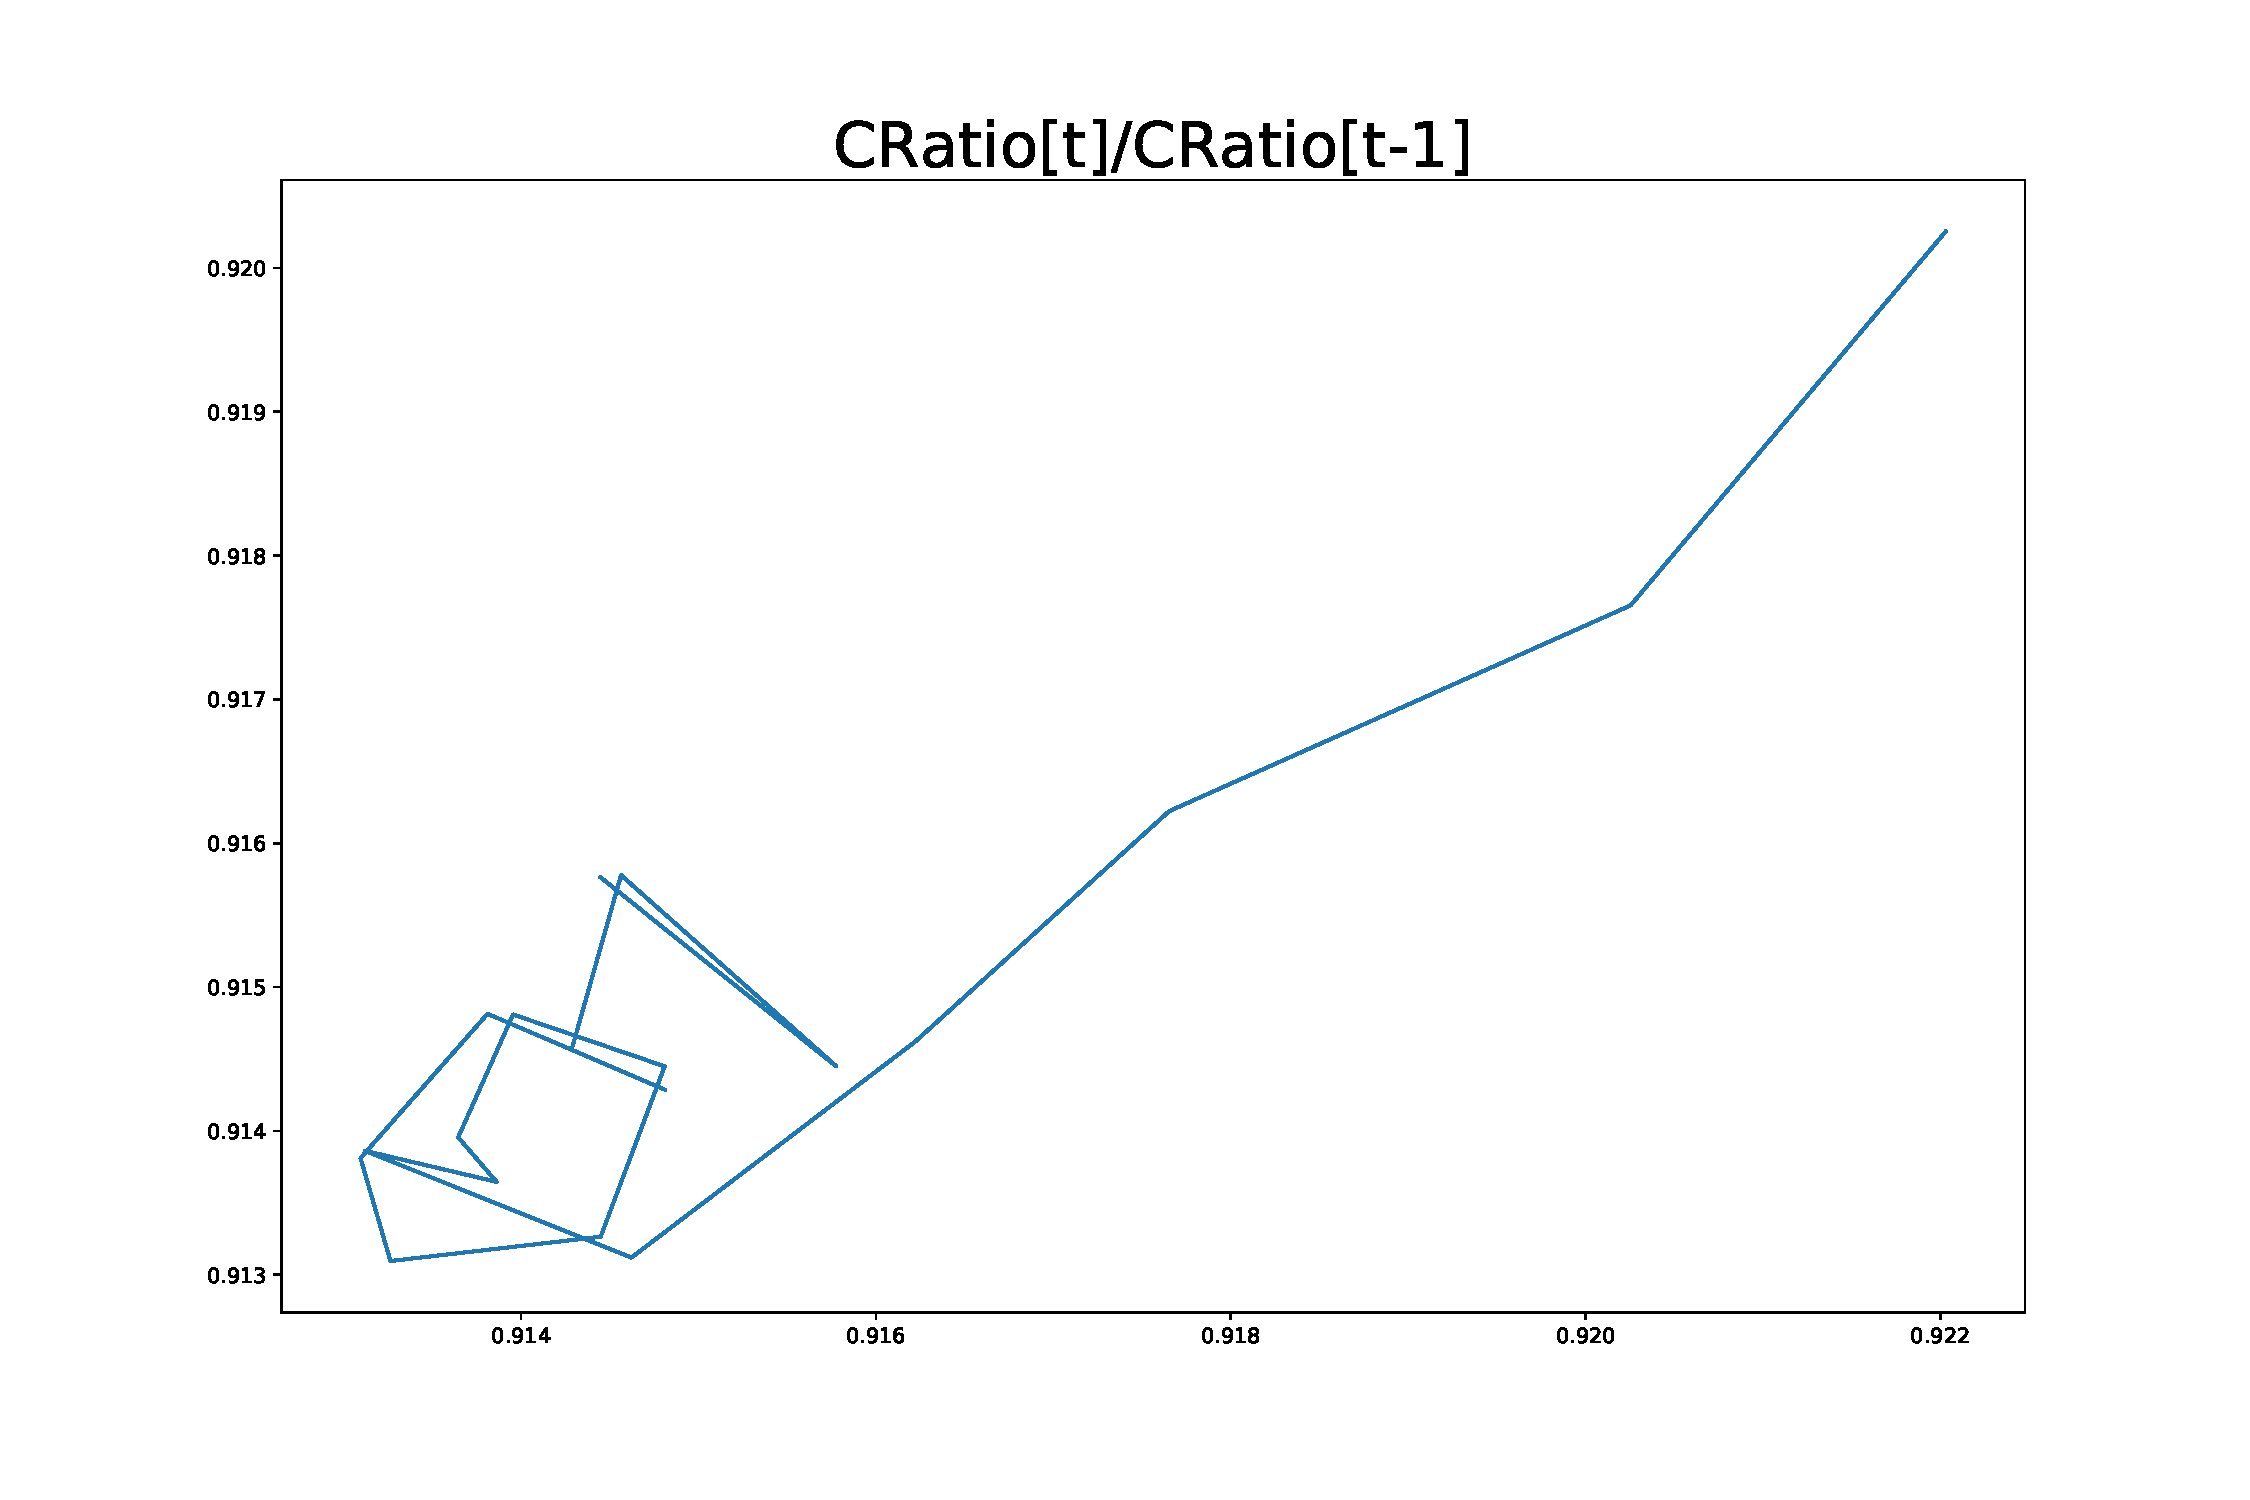
\includegraphics[width=1.2\textwidth]{../50kSample_BaseCal/CRatio.pdf}
		\caption{Sample 50k, tol = 1E-3}
		\label{fig:Cratio-50k-Baseline}
	\end{subfigure}
	\hfill
	\begin{subfigure}[b]{0.45\textwidth}
		\centering
		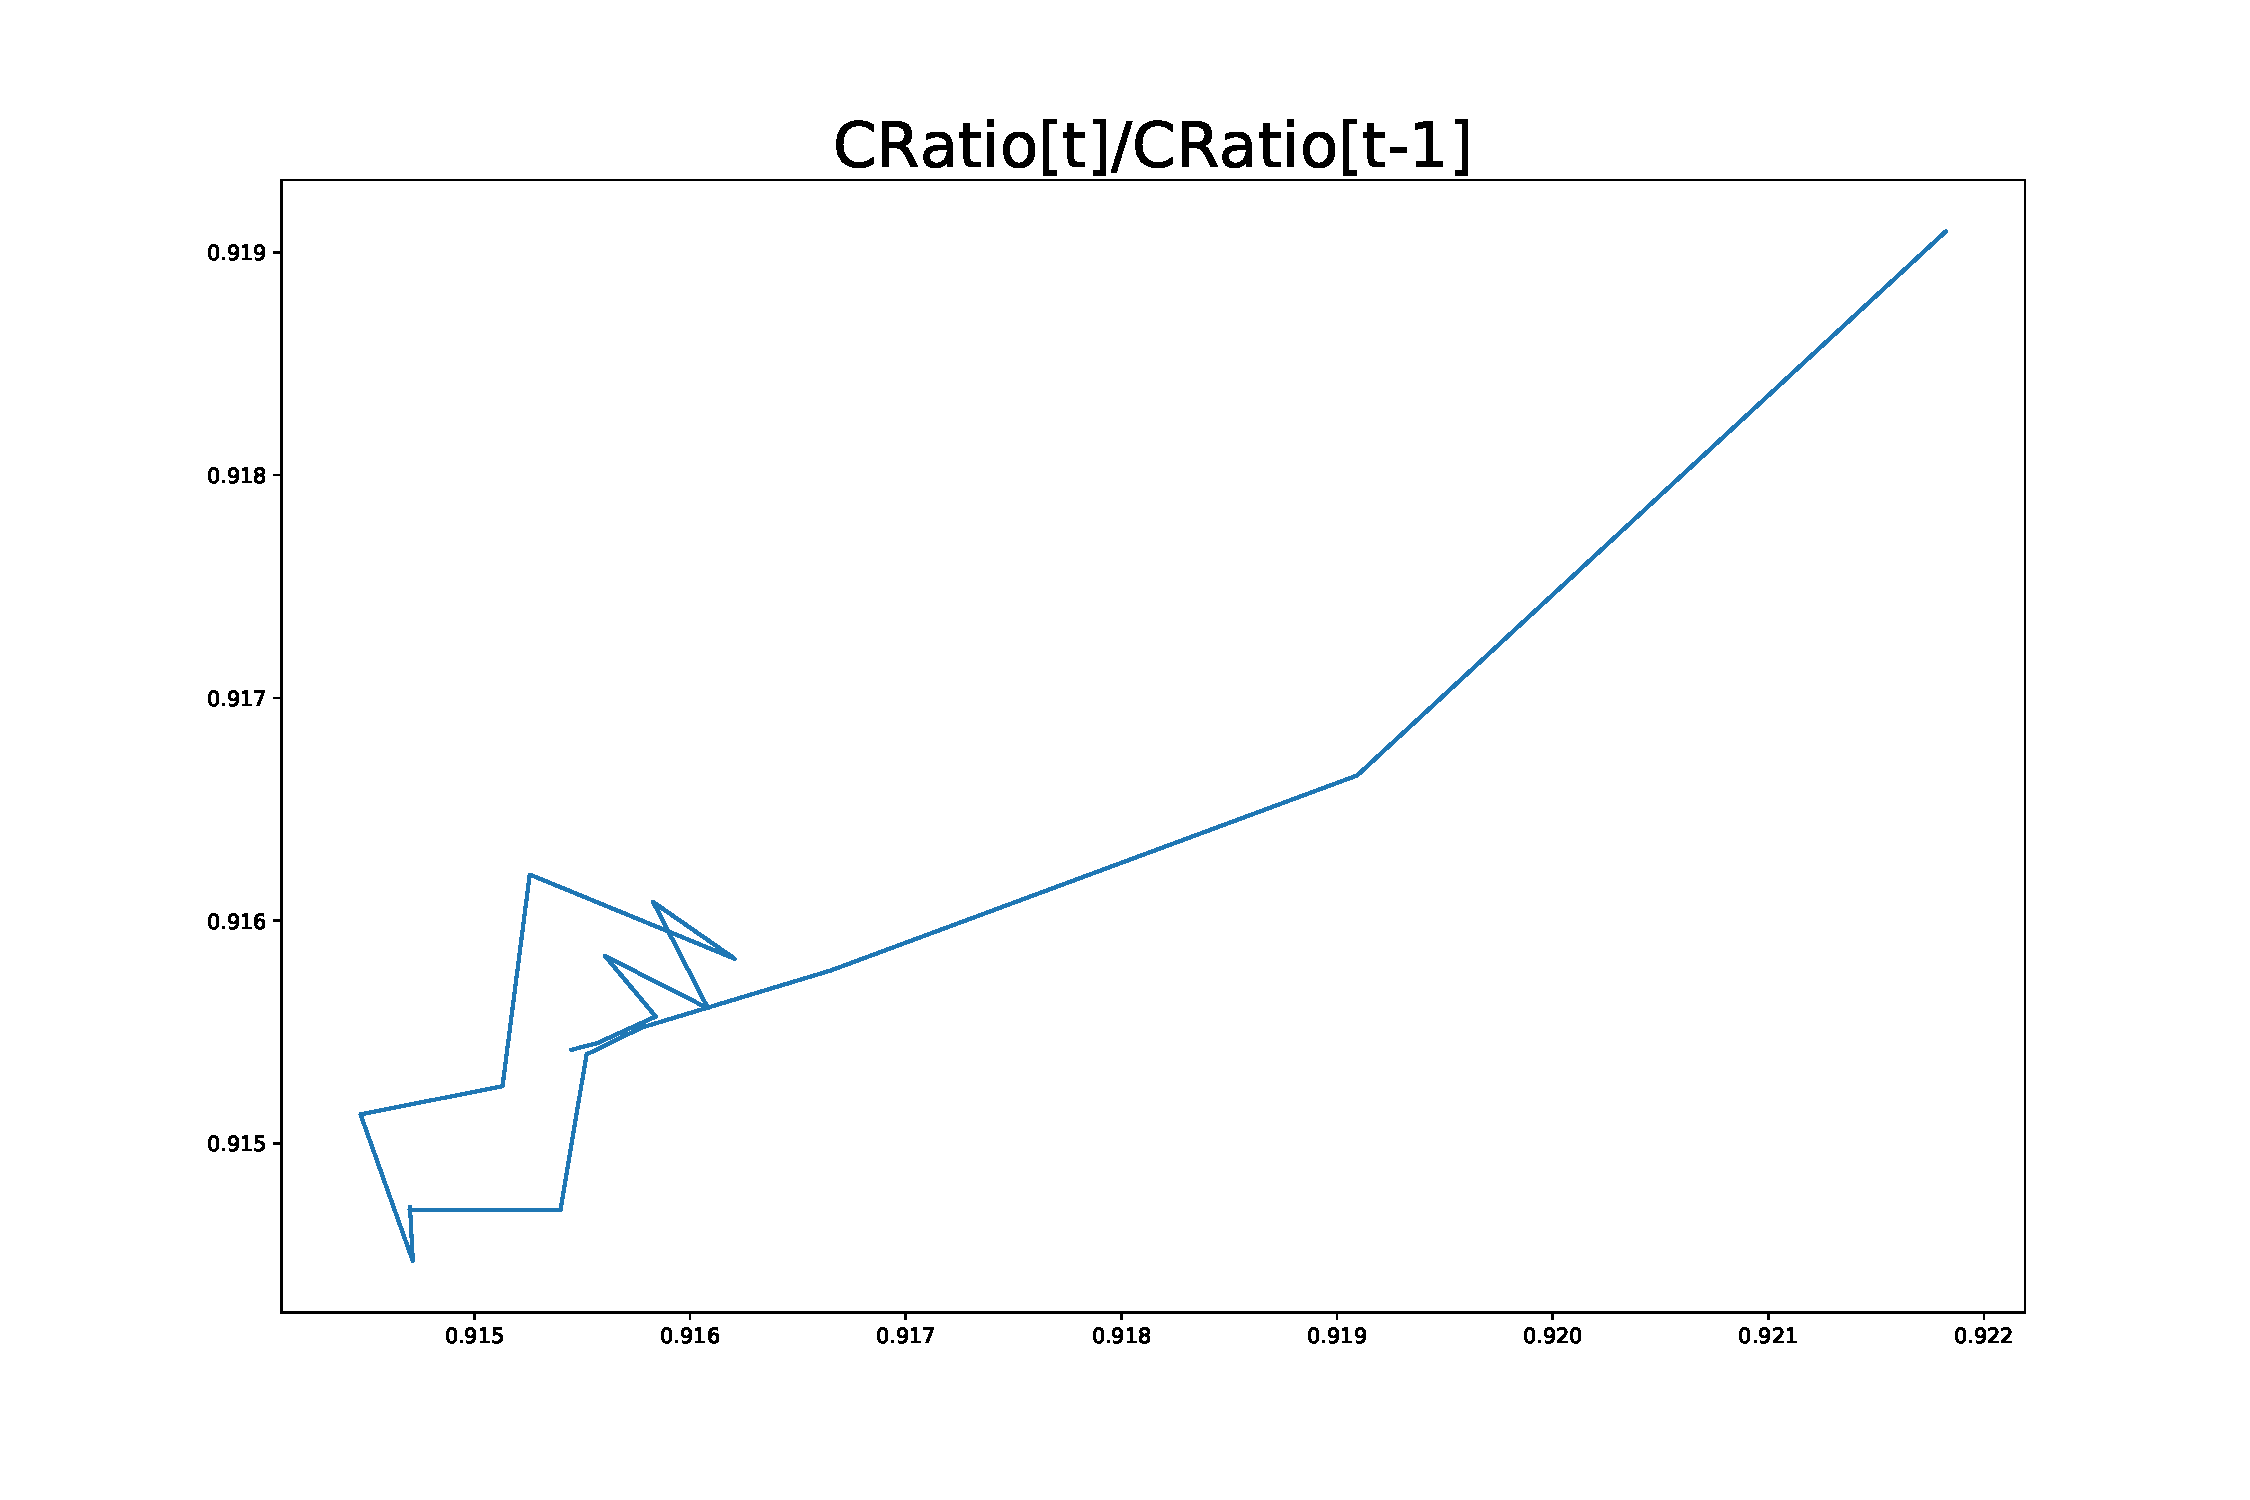
\includegraphics[width=1.2\textwidth]{../200kSample_BaseCal/CRatio.pdf}
		\caption{Sample 200k, tol = 1E-3}
		\label{fig:Cratio-200k-Baseline}
	\end{subfigure}\\
	\begin{subfigure}[b]{0.45\textwidth}
		\centering
		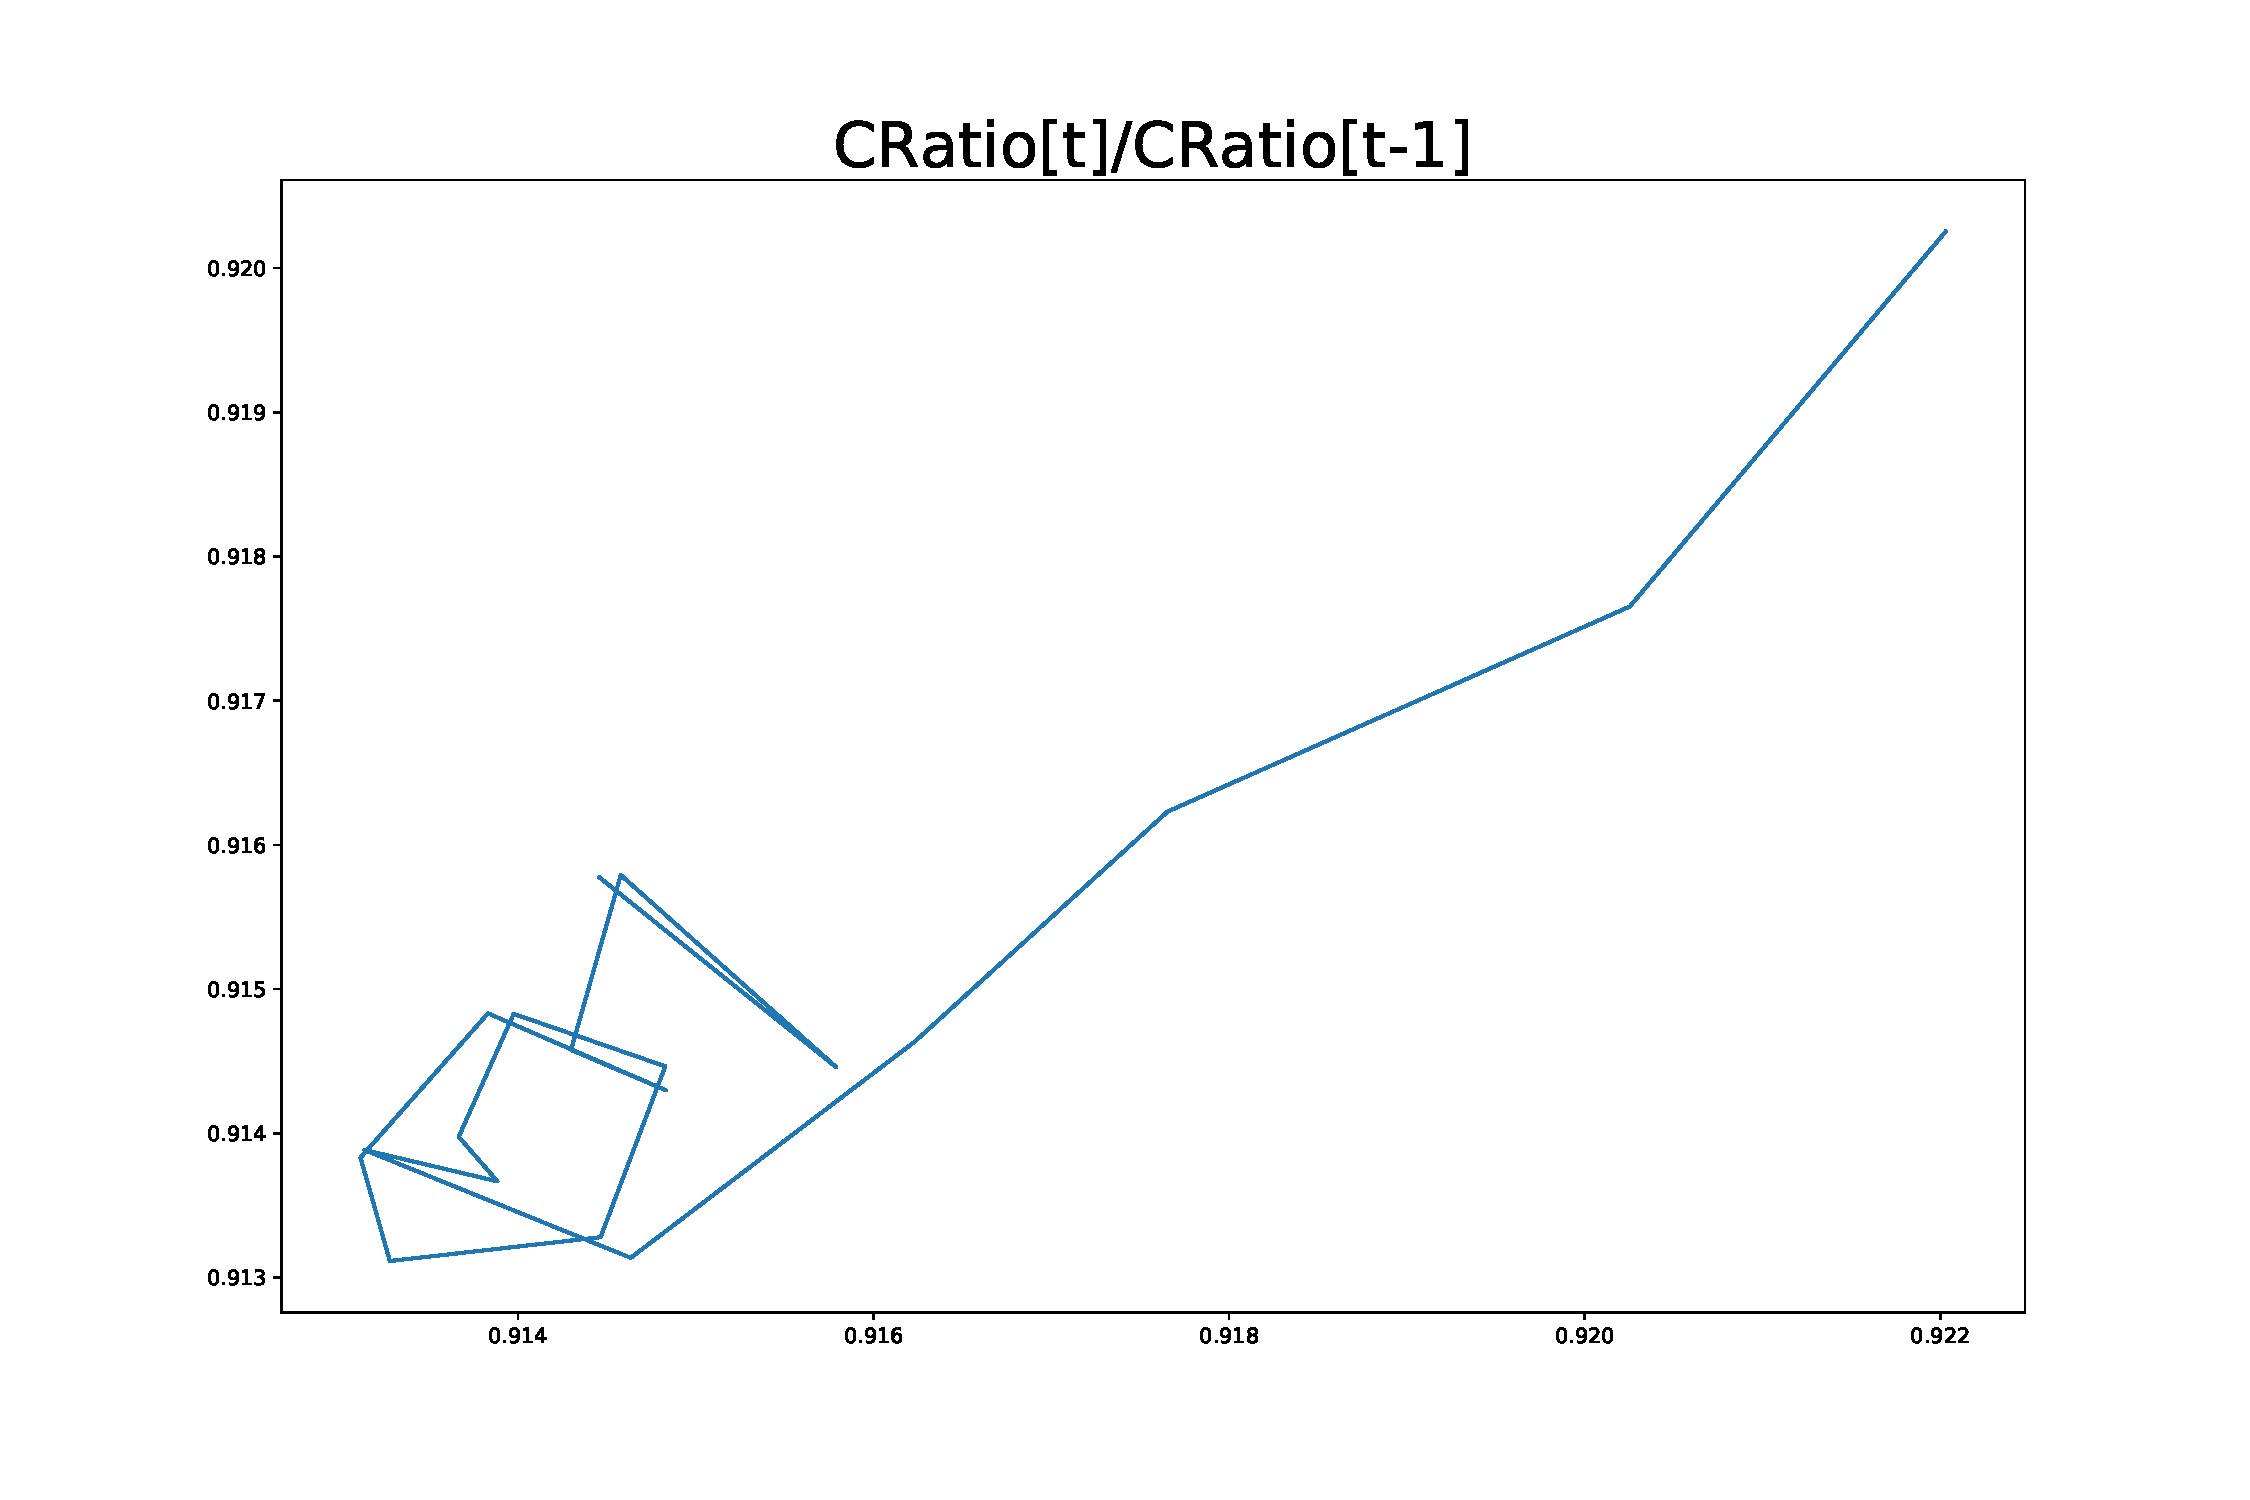
\includegraphics[width=1.2\textwidth]{../50kSample_BaseCal_TolE-4/CRatio.pdf}
		\caption{Sample 50k, tol = 1E-4}
		\label{fig:Cratio-50k}
	\end{subfigure}
	\hfill
	\begin{subfigure}[b]{0.45\textwidth}
		\centering
		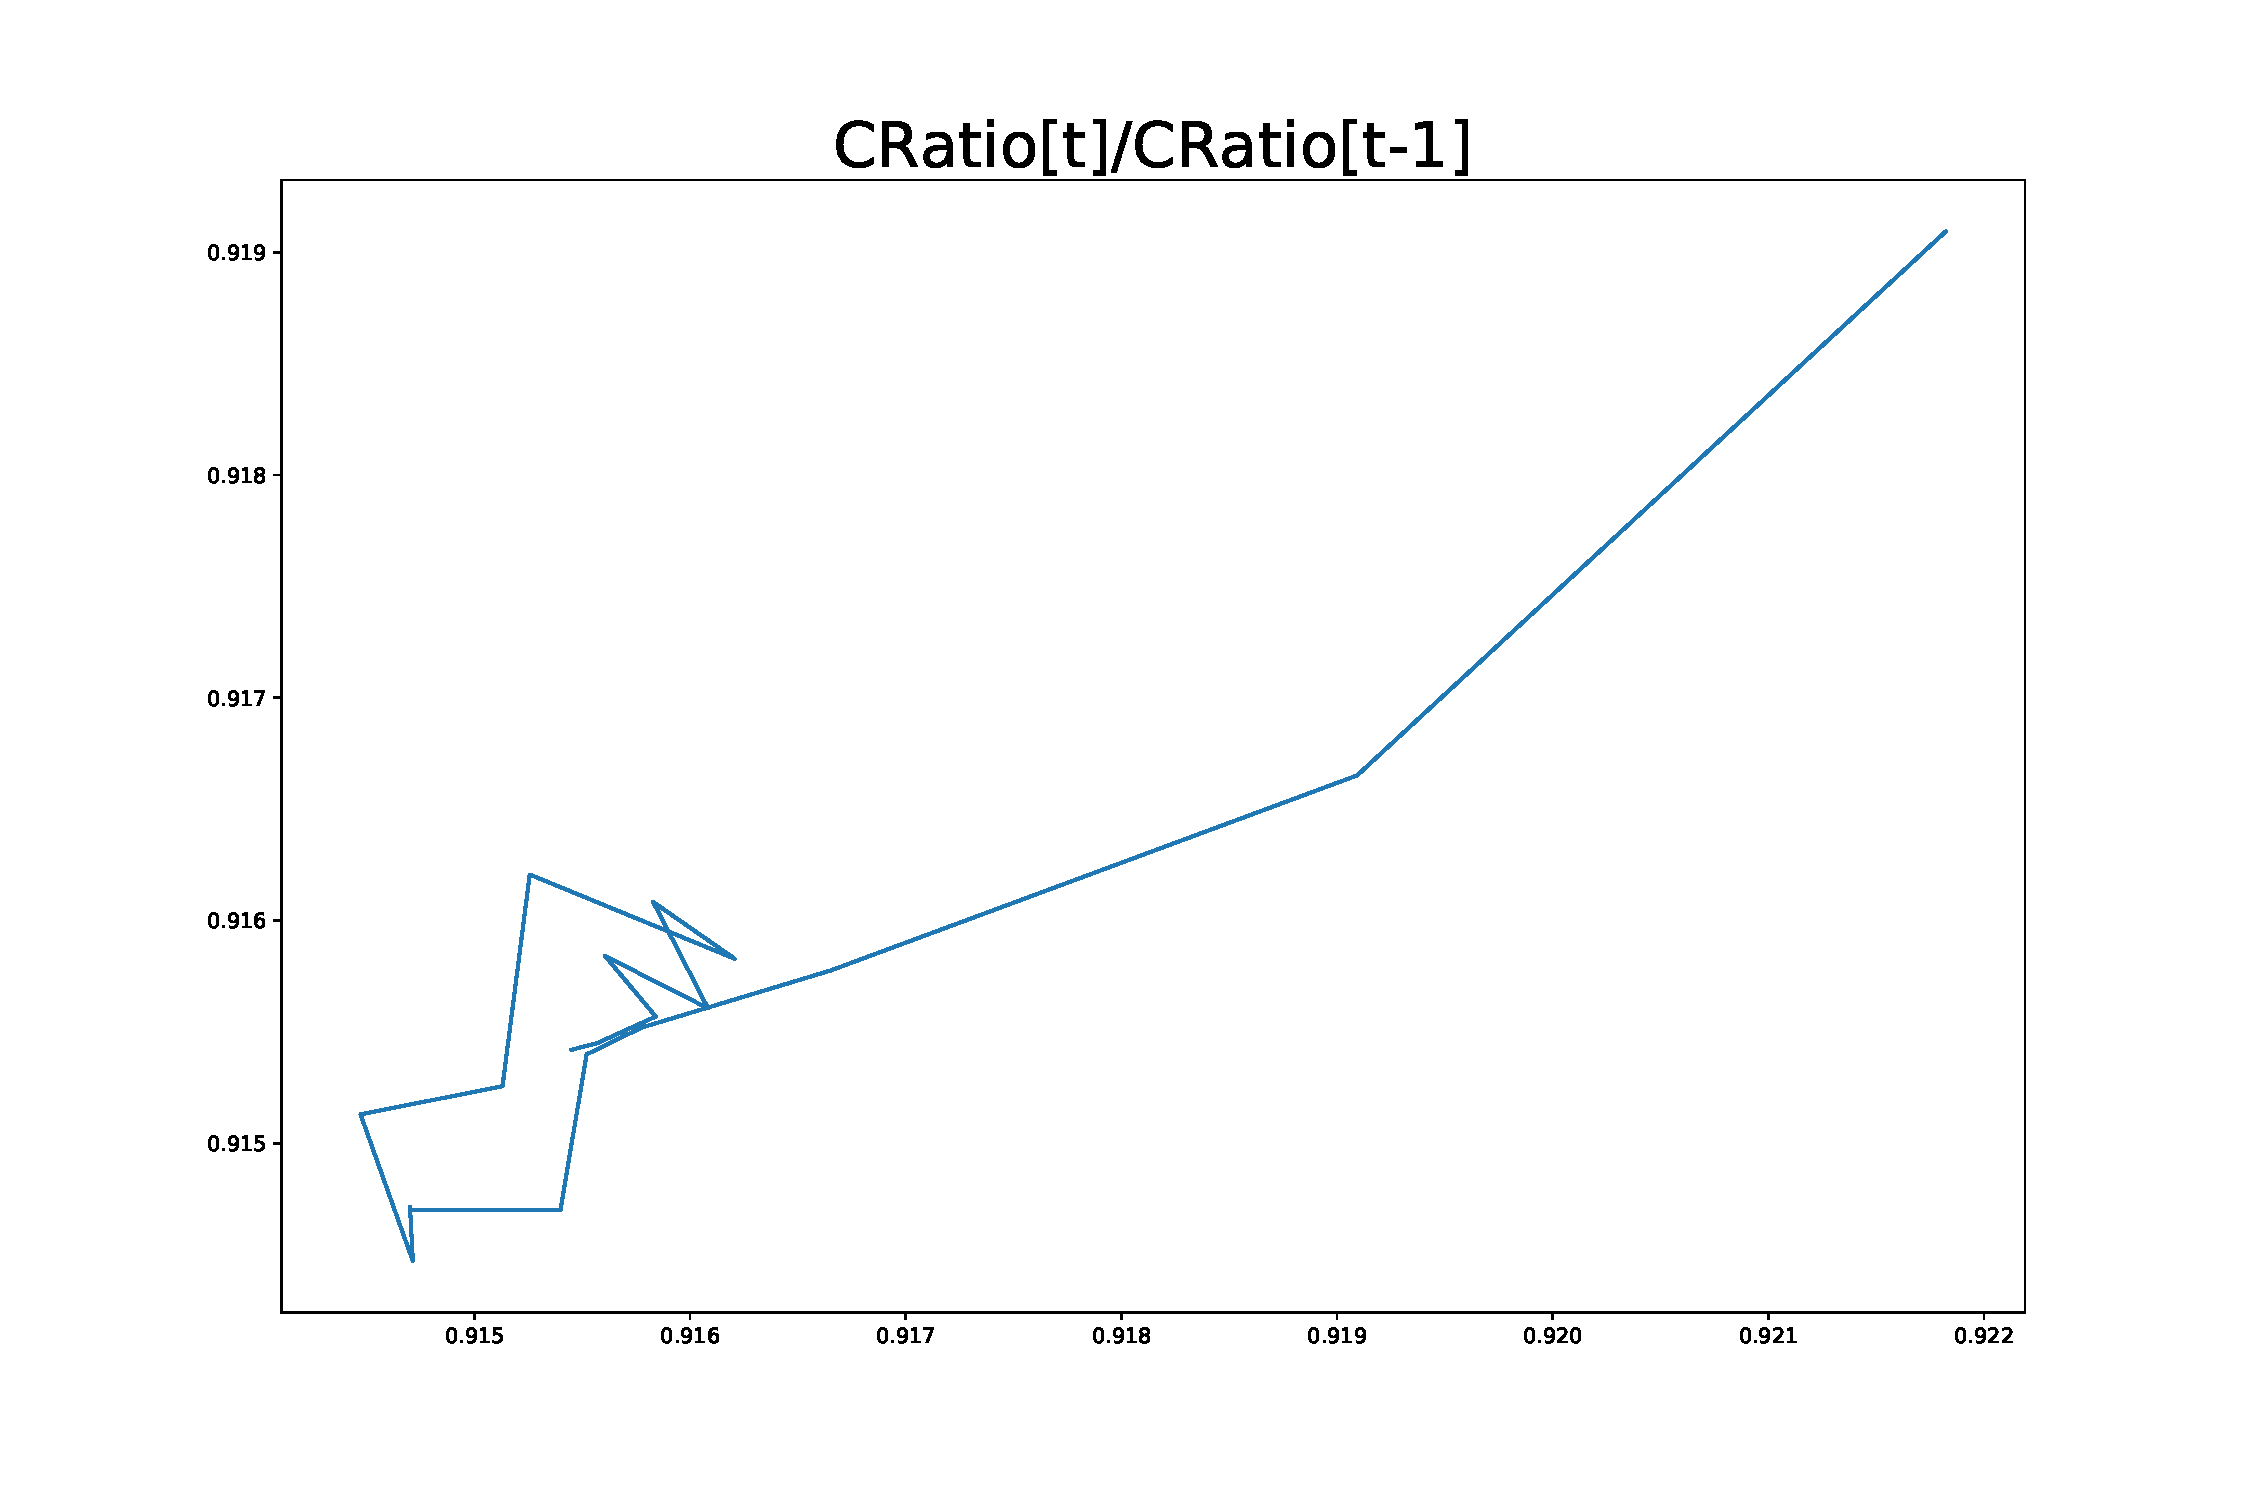
\includegraphics[width=1.2\textwidth]{../200kSample_BaseCal_TolE-4/CRatio.pdf}
		\caption{Sample 200k, tol = 1E-4}
		\label{fig:Cratio-200k}
	\end{subfigure}
	\caption{Plotting $CR_t$ (y-axis) on $CR_{t-1}$ (x-axis). (subfigure's title misleading, please ignore)}
	\label{fig:CRatio}
\end{figure}








\end{document}
